% piano di progetto
% da compilare con il comando pdflatex Esterni/Piano_di_progetto/Piano_di_progetto_v_x.x.x.tex

% Dichiarazioni di ambiente e inclusione di pacchetti
% da usare tramite il comando % Dichiarazioni di ambiente e inclusione di pacchetti
% da usare tramite il comando % Dichiarazioni di ambiente e inclusione di pacchetti
% da usare tramite il comando \input{../../util/hx-ambiente}

\documentclass[a4paper,titlepage]{article}
\usepackage[T1]{fontenc}
\usepackage[utf8]{inputenc}
\usepackage[english,italian]{babel}
\usepackage{microtype}
\usepackage{lmodern}
\usepackage{underscore}
\usepackage{graphicx}
\usepackage{eurosym}
\usepackage{float}
\usepackage{fancyhdr}
\usepackage[table]{xcolor}
\usepackage{longtable}
\usepackage{chngpage}
\usepackage{grffile}
\usepackage[titles]{tocloft}
\usepackage{hyperref}
\hypersetup{hidelinks}

\usepackage{../../util/hx-vers}
\usepackage{../../util/hx-macro}
\usepackage{../../util/hx-front}

% solo se si vuole una nuova pagina ad ogni \section:
\usepackage{titlesec}
\newcommand{\sectionbreak}{\clearpage}

% stile di pagina:
\pagestyle{fancy}

% solo se si vuole eliminare l'indentazione ad ogni paragrafo:
\setlength{\parindent}{0pt}

% intestazione:
\lhead{\Large{\proj}}
\rhead{
\includegraphics[keepaspectratio=true,width=50px]{../../util/hivex_logo2.png}}
\renewcommand{\headrulewidth}{0.4pt}

% pie' di pagina:
\lfoot{\email}
\rfoot{\thepage}
\cfoot{}
\renewcommand{\footrulewidth}{0.4pt}

% spazio verticale tra le celle di una tabella:
\renewcommand{\arraystretch}{1.5}

% profondità di indicizzazione:
\setcounter{tocdepth}{4}
\setcounter{secnumdepth}{4}


\documentclass[a4paper,titlepage]{article}
\usepackage[T1]{fontenc}
\usepackage[utf8]{inputenc}
\usepackage[english,italian]{babel}
\usepackage{microtype}
\usepackage{lmodern}
\usepackage{underscore}
\usepackage{graphicx}
\usepackage{eurosym}
\usepackage{float}
\usepackage{fancyhdr}
\usepackage[table]{xcolor}
\usepackage{longtable}
\usepackage{chngpage}
\usepackage{grffile}
\usepackage[titles]{tocloft}
\usepackage{hyperref}
\hypersetup{hidelinks}

\usepackage{../../util/hx-vers}
\usepackage{../../util/hx-macro}
\usepackage{../../util/hx-front}

% solo se si vuole una nuova pagina ad ogni \section:
\usepackage{titlesec}
\newcommand{\sectionbreak}{\clearpage}

% stile di pagina:
\pagestyle{fancy}

% solo se si vuole eliminare l'indentazione ad ogni paragrafo:
\setlength{\parindent}{0pt}

% intestazione:
\lhead{\Large{\proj}}
\rhead{
\includegraphics[keepaspectratio=true,width=50px]{../../util/hivex_logo2.png}}
\renewcommand{\headrulewidth}{0.4pt}

% pie' di pagina:
\lfoot{\email}
\rfoot{\thepage}
\cfoot{}
\renewcommand{\footrulewidth}{0.4pt}

% spazio verticale tra le celle di una tabella:
\renewcommand{\arraystretch}{1.5}

% profondità di indicizzazione:
\setcounter{tocdepth}{4}
\setcounter{secnumdepth}{4}


\documentclass[a4paper,titlepage]{article}
\usepackage[T1]{fontenc}
\usepackage[utf8]{inputenc}
\usepackage[english,italian]{babel}
\usepackage{microtype}
\usepackage{lmodern}
\usepackage{underscore}
\usepackage{graphicx}
\usepackage{eurosym}
\usepackage{float}
\usepackage{fancyhdr}
\usepackage[table]{xcolor}
\usepackage{longtable}
\usepackage{chngpage}
\usepackage{grffile}
\usepackage[titles]{tocloft}
\usepackage{hyperref}
\hypersetup{hidelinks}

\usepackage{../../util/hx-vers}
\usepackage{../../util/hx-macro}
\usepackage{../../util/hx-front}

% solo se si vuole una nuova pagina ad ogni \section:
\usepackage{titlesec}
\newcommand{\sectionbreak}{\clearpage}

% stile di pagina:
\pagestyle{fancy}

% solo se si vuole eliminare l'indentazione ad ogni paragrafo:
\setlength{\parindent}{0pt}

% intestazione:
\lhead{\Large{\proj}}
\rhead{
\includegraphics[keepaspectratio=true,width=50px]{../../util/hivex_logo2.png}}
\renewcommand{\headrulewidth}{0.4pt}

% pie' di pagina:
\lfoot{\email}
\rfoot{\thepage}
\cfoot{}
\renewcommand{\footrulewidth}{0.4pt}

% spazio verticale tra le celle di una tabella:
\renewcommand{\arraystretch}{1.5}

% profondità di indicizzazione:
\setcounter{tocdepth}{4}
\setcounter{secnumdepth}{4}

\version{0.0.5}
\creaz{25 dicembre 2016}
\author{\LB, \PB}
\supervisor{\GG, \MM}
\uso{esterno}
\dest{\TV, \ZU}
\title{Piano di progetto}

\begin{document}
\maketitle
% diario delle modifiche per il piano di progetto
% da includere con % diario delle modifiche per il piano di progetto
% da includere con % diario delle modifiche per il piano di progetto
% da includere con \include{diario}

\begin{diario}
	1.0.1 & {\GG} (Responsabile) & 03/02/2017 & Correzione degli errori individuati nelle prime tre sezioni del documento \\ \hline
	1.0.0 & {\PB} (Responsabile) & 09/01/2017 & Approvazione documento \\ \hline
	0.1.0 & {\MM} (Verificatore) & 07/01/2017 & Verifica documento \\ \hline
	0.0.9 & {\PB} (Responsabile) & 05/01/2017 & Stesura Organigramma \\ \hline
	0.0.8 & {\LB} (Responsabile) & 05/01/2017 & Stesura Consuntivo di Periodo \\ \hline
	0.0.7 & {\LB} (Responsabile) & 04/01/2017 & Stesura Preventivo di Periodo \\ \hline
	0.0.6 & {\LB} (Responsabile) & 03/01/2017 & Inserimento Gantt Diagrammi delle Attività \\ \hline
	0.0.5 & {\PB} (Responsabile) & 29/12/2016 & Stesura Pianificazione delle Attività \\ \hline
	0.0.4 & {\PB} (Responsabile) & 28/12/2016 & Stesura Introduzione \\ \hline
	0.0.3 & {\LB} (Responsabile) & 27/12/2016 & Stesura Modello di sviluppo \\ \hline
	0.0.2 & {\PB} (Responsabile) & 27/12/2016 & Stesura Analisi dei Rischi \\ \hline
	0.0.1 & {\LB} (Responsabile) & 26/12/2016 & Stesura scheletro \\ \hline
\end{diario}

\begin{diario}
	1.0.1 & {\GG} (Responsabile) & 03/02/2017 & Correzione degli errori individuati nelle prime tre sezioni del documento \\ \hline
	1.0.0 & {\PB} (Responsabile) & 09/01/2017 & Approvazione documento \\ \hline
	0.1.0 & {\MM} (Verificatore) & 07/01/2017 & Verifica documento \\ \hline
	0.0.9 & {\PB} (Responsabile) & 05/01/2017 & Stesura Organigramma \\ \hline
	0.0.8 & {\LB} (Responsabile) & 05/01/2017 & Stesura Consuntivo di Periodo \\ \hline
	0.0.7 & {\LB} (Responsabile) & 04/01/2017 & Stesura Preventivo di Periodo \\ \hline
	0.0.6 & {\LB} (Responsabile) & 03/01/2017 & Inserimento Gantt Diagrammi delle Attività \\ \hline
	0.0.5 & {\PB} (Responsabile) & 29/12/2016 & Stesura Pianificazione delle Attività \\ \hline
	0.0.4 & {\PB} (Responsabile) & 28/12/2016 & Stesura Introduzione \\ \hline
	0.0.3 & {\LB} (Responsabile) & 27/12/2016 & Stesura Modello di sviluppo \\ \hline
	0.0.2 & {\PB} (Responsabile) & 27/12/2016 & Stesura Analisi dei Rischi \\ \hline
	0.0.1 & {\LB} (Responsabile) & 26/12/2016 & Stesura scheletro \\ \hline
\end{diario}

\begin{diario}
	1.0.1 & {\GG} (Responsabile) & 03/02/2017 & Correzione degli errori individuati nelle prime tre sezioni del documento \\ \hline
	1.0.0 & {\PB} (Responsabile) & 09/01/2017 & Approvazione documento \\ \hline
	0.1.0 & {\MM} (Verificatore) & 07/01/2017 & Verifica documento \\ \hline
	0.0.9 & {\PB} (Responsabile) & 05/01/2017 & Stesura Organigramma \\ \hline
	0.0.8 & {\LB} (Responsabile) & 05/01/2017 & Stesura Consuntivo di Periodo \\ \hline
	0.0.7 & {\LB} (Responsabile) & 04/01/2017 & Stesura Preventivo di Periodo \\ \hline
	0.0.6 & {\LB} (Responsabile) & 03/01/2017 & Inserimento Gantt Diagrammi delle Attività \\ \hline
	0.0.5 & {\PB} (Responsabile) & 29/12/2016 & Stesura Pianificazione delle Attività \\ \hline
	0.0.4 & {\PB} (Responsabile) & 28/12/2016 & Stesura Introduzione \\ \hline
	0.0.3 & {\LB} (Responsabile) & 27/12/2016 & Stesura Modello di sviluppo \\ \hline
	0.0.2 & {\PB} (Responsabile) & 27/12/2016 & Stesura Analisi dei Rischi \\ \hline
	0.0.1 & {\LB} (Responsabile) & 26/12/2016 & Stesura scheletro \\ \hline
\end{diario}
\tableofcontents
\newpage

\section{Introduzione}
	\subsection{Scopo del documento}.

	Il presente documento illustra la pianificazione adottata dal gruppo \hx{} finalizzata alla produzione del progetto \proj{}. Esso è suddiviso nelle seguenti sezioni:
\begin{description}
	\item[sezione \ref{sec:modello}] Scelta del modello di sviluppo adottato;
	\item[sezione \ref{sec:analisi}] Analisi e trattamento dei rischi;
	\item[sezione \ref{sec:pianificazione}] Pianificazione delle attività;
	\item[sezione \ref{sec:preventivo}] Suddivisione delle ore lavorative e preventivo;
           \item[sezione \ref{sec:consuntivo}] Consuntivo di periodo;
	\item[sezione \ref{sec:organigramma}] Organigramma.
\end{description}

	\subsection{Scopo del prodotto}
	\scopo{}
	
	\subsection{Glossario}
	\presgloss{}
	\subsection{Riferimenti}
		\subsubsection{Normativi}
		\begin{description}
			\item \NdP;
			\item[Capitolato d'appalto C6: \proj]\url{http://www.math.unipd.it/~tullio/IS-1/2016/Progetto/C6p.pdf};
			\item[Regolamento del progetto didattico]\url{http://www.math.unipd.it/~tullio/IS-1/2016/Dispense/L09.pdf};
			\item[Vincoli di organigramma e dettagli tecnico-economici]\url{http://www.math.unipd.it/~tullio/IS-1/2016/Progetto/PD01b.html}.
		\end{description}
		\subsubsection{Informativi} \label{sec:ref}
		\begin{description}
			\item[Slides del corso di Ingegneria del Software]\url{http://www.math.unipd.it/~tullio/IS-1/2016/};
			\item[Ingegneria del Software - Ian Sommerville - Ottava Edizione]
			\begin{itemize}
				\item Capitolo 4: Software Processes;
			\end{itemize}
		\end{description}

	\subsection{Scadenze}
	Il gruppo \hx{} ha deciso di rispettare le seguenti scadenze:
		\begin{description}
			\item[Revisione dei Requisiti] 24-01-2017;
			\item[Revisione di Progettazione] 13-03-2017 presentandosi con Revisione di Progettazione minima;
			\item[Revisione di Qualifica] 18-04-2017;
			\item[Revisione di Accettazione] 15-05-2017.
		\end{description}


\section{Modello di sviluppo} \label{sec:modello}

	La scelta di un modello di sviluppo è cruciale per la corretta pianificazione delle attività. Da essa infatti si deriva tutta la struttura principale con cui saranno pianificati milestone e task.

	Il progetto {\proj}, come affrontato nei documenti \emph{Studio di fattibilità} e \emph{Piano di Qualifica}, presenta numerosi punti critici, analizzati nella sezione {\ref{sec:analisi}}, in particolare nella sezione {\ref{sec:tec}}, in cui sono analizzati i rischi tecnologici. Generalmente {\proj} richiede una intensiva fase di progettazione, il cui fine ultimo è l'esplorazione delle problematiche legate ai software \gloss{CASE} e alla loro risoluzione, tenendo conto del quantitativo di risorse assegnate al progetto. %[riferimento a verbale di riunione con zucchetti?]

	Un progetto dedito all'esplorazione va supportato con un adeguato modello di sviluppo; esso deve avere i seguenti requisiti:

	\begin{itemize}
		\item \textbf{Tracciabilità delle funzionalità di massima del software}, per definire gli obiettivi cardine del progetto;
		\item Sufficiente \textbf{elasticità in fase di progettazione}, al fine di poter esplorare in modo profondo le possibili implementazioni;
		\item Possibilità di \textbf{raffinamento dei requisiti}, in caso si volesse indirizzare la ricerca in una direzione piuttosto che un'altra, con il vincolo di dover definire fin da subito i soli requisiti obbligatori;
		\item \textbf{Validazione del software} prodotto, per poter garantire le funzionalità concordate.
	\end{itemize}

	Di seguito vengono analizzati sinteticamente punti deboli e punti di forza dei principali approcci ai processi software, nel contesto del nostro progetto.
	
	Va tuttavia ricordato che non è sconsigliato adottare più modelli in forma ibrida, come suggerito da Sommerville (vedi \ref{sec:ref}).

	\subsection{Analisi modelli di sviluppo}

		\subsubsection{Modelli di sviluppo sequenziale}

			\paragraph{Modello a cascata}

			Il modello a cascata (Royce, 1970) è il più antico dei modelli software analizzati e fondamentalmente identifica cinque attività di sviluppo principali:
			
\begin{description}
\item [Analisi e definizione dei requisiti] il problema viene ben definito, specificando obiettivi e vincoli;
\item [Progettazione del sistema] si stabilisce una architettura software;
\item [Implementazione e test di unità] sono sviluppati una serie di unità e i loro relativi test;
\item [Integrazione e test di sistema] le singole unità sono integrate e sono effettuati test di sistema che devono soddisfare le specifiche iniziali;
\item [Manuntenzione] la fase del ciclo di vita auspicabilmente più longeva.
\end{description}
			
			Questo tipo di approccio:
\begin{itemize}
\item Promette un prodotto finito, con grande attenzione alle deadline tracciate inizialmente;
\item Stabilisce una architettura software iniziale stabile.
\end{itemize}

			Di contro, i svantaggi di questo approccio sono svariati:
\begin{itemize}
\item Le varie fasi sono a compartimenti stagni: una volta tracciati i requisiti, essi non possono più venire modificati.
\item Il committente deve avere già inizialmente una idea molto chiara del prodotto che desidera. 
\end{itemize}

Questi ultimi punti entrano in netto contrasto con i requisiti inizialmente proposti; ciò ha portato a scartare questo modello di sviluppo. Tuttavia adotteremo una politica a deadline, anche a causa dei vincoli imposti dalle revisioni del {\TV}.

			\paragraph{Modello evolutivo}

			Il modello evolutivo, particolarmente apprezzato da Sommerville, prevede una implementazione iniziale e una forte collaborazione tra committente e fornitore allo scopo di raffinare il sistema tramite più versioni del prodotto, fino a raggiungere un sistema adeguato alle esigenze dell'utente.

Ciò si può realizzare principalmente tramite due strumenti differenti: lo \emph{exploratory development} e il \emph{throwaway prototyping}.

Il primo consiste nel lavorare a fianco del cliente per esplorare i suoi requisiti e infine consegnare un sistema adeguato. Mentre questo metodo di lavoro potrebbe sembrare positivo, esso presenta due grosse criticità: 
\begin{itemize}
\item Cambiamenti continui tendono a corrompere la struttura e l'architettura del software;
\item Aggiungere estensioni non previste diventa progressivamente più complesso e costoso. 
\end{itemize}
Questo rischio a parere di \hx{} non riesce ad essere bilanciato dalla possibilità di ritardare requisiti e decisioni di design.

La seconda possibilità invece consiste nell'avere dei prototipi usati per meglio comprendere il problema. La criticità presente riguarda il futuro di questi prototipi: sviluppare un prototipo porta valore esclusivamente nell'ambito di comprensione i requisiti del progetto, non porta un effettivo avanzamento nello sviluppo del prodotto.

			\paragraph{Modello basato su componenti}
Questo modello si basa sull'approccio orientato al riuso di componenti già esistenti, in modo da abbattere tempi e costi.

Esso si differenzia per alcuni differenti fasi intermedie orientate al riuso:

\begin{description}
\item [Analisi dei componenti] a partire dalla specifica dei requisiti, sono ricercati delle componenti già esistenti che possano soddisfare la specifica esistente.
\item [Modifica dei requisiti] i requisiti variano a seconda delle componenti che sono state identificate.
\item [Progettazione del sistema con riuso] viene tracciata l'architettura del sistema e sono progettate in dettaglio le componenti non disponibili al riuso.
\item [Sviluppo e integrazione] Sono sviluppate le componenti non esistenti ed esse sono integrate al sistema con riuso. L'integrazione e lo sviluppo possono non essere attività separate.

\end{description}
Questo approccio è sicuramente interessante e, malgrado non sia stato adottato in toto, ci si riserva la possibilità di seguire i punti che prevedono il design del sistema con riuso e una modifica dei requisiti, al fine di ridurre i tempi e costi di certe componenti del sistema. \hx{} ritiene inoltre che gli svantaggi riguardo ai compromessi che nasceranno siano di gran lunga ripagati dai benefici di questo approccio; infine l'approccio è stato approvato dal committente in sede di discussione.

		\subsubsection{Modelli di sviluppo iterativi}
			\paragraph{Modello incrementale}
			Questo modello sfrutta un approccio che vuole combinare i vantaggi del modello a cascata con il modello evolutivo. Essenzialmente si prevede che il committente identifichi le componenti più importanti e meno importanti; quindi si sviluppa una architettura di base e si fissano degli incrementi delle funzionalità del sistema in iterazioni successive.

Questo modello richiede che ogni incremento:
\begin{itemize}
\item Apporti funzionalità tangibili;
\item Non deve essere eccessivamente ampio (<20mila righe di codice)
\item Sia validato singolarmente, integrato e sia validato nel complesso
\end{itemize}

I vantaggi di questo modello sono molteplici:
\begin{itemize}
\item Permette di sperimentare il sistema con il committente al fine di chiarificare tutti i requisiti;
\item I primi incrementi possono essere usati come prototipi;
\item I servizi a più alta priorità passano inevitabilmente il maggior numero di fasi di test.
\end{itemize}

Vanno segnalati tuttavia i seguenti difetti:
\begin{itemize}
\item Può essere difficile trasformare i requisiti del cliente in incrementi di una misura adeguata;
\item Non è possibile modificare i requisiti già esistenti negli incrementi successivi.
\end{itemize}

Ciò si traduce in una criticità del processo nella fase di analisi. Nella sezione {\ref{sec:analisi}} (Analisi dei rischi) si analizza come questo rischio verrà trattato.

In complesso, \hx{} ritiene che il modello incrementale apporti sostanziali vantaggi rispetto agli altri modelli finora analizzati. In seguito si analizzano altri modelli che sono stati presi in considerazione.

			\paragraph{Modello a spirale}
			Il modello a spirale (Boehm, 1988) è un approccio fondamentalmente rappresentato come una sequenza di attività che si ripetono nel tempo, partendo dalla fattibilità, definizione dei requisiti, ideazione dell'architettura, e così via.
			
			Le quattro operazioni ripetute all'interno della spirale sono:
\begin{itemize}
\item Identificazione degli obiettivi
\item Valutazione del rischio
\item Sviluppo e validazione
\item Pianificazione (della fase successiva)
\end{itemize}			 

L'approccio sfrutta una metodologia fortemente \emph{risk-driven} che, malgrado possa portare dei benefici al prodotto finale, essa rischierebbe di appesantire eccessivamente il team, il processo di sviluppo e le risorse.


\newpage \section{Analisi dei rischi} \label{sec:analisi}
In questa sezione del documento vengono elencati e descritti tutti i possibili rischi che potrebbero colpire il gruppo \hx{} nella realizzazione del prodotto \proj. Per gestire tali rischi, è stata attuata la seguente procedura che prevede:
\begin{description}
	\item[Identificazione dei rischi] trovare i rischi potenziali che si possono presentare durante l'intero sviluppo del progetto e studiarne la natura. Essi possono essere di tre tipologie:
	\begin{description}
		\item[Progetto] relativi a pianificazione, strumenti e risorse;
		\item[Prodotto] relativi a conformità e aspettative del committente;
		\item[Business] relativi a costi e concorrenza.
	\end{description}
	\item[Analisi dei rischi] studiare per ogni rischio le:
	\begin{description}
		\item[Probabilità di occorrenza];
		\item[Conseguenze] comprendere che peso hanno sul progetto per comprenderne le criticità.
	\end{description}
	\item[Pianificazione di controllo e mitigazione] istituire metodi di controllo per i rischi, così da poterli evitare facendo:
	\begin{description}
		\item[Verifica costante del livello di rischio];
		\item[Riconoscimento e trattamento].
	\end{description}
	\item[Attuazione nel periodo] viene progressivamente descritto se il rischio si è verificato e in tal caso, in che modo il gruppo ha reagito e cosa ha comportato.
\end{description}
Ciascun rischio viene identificato a:
\begin{description}
	\item[Livello tecnologico](sezione \ref{sec:tec});
	\item[Livello del personale](sezione \ref{sec:per});
	\item[Livello organizzativo](sezione \ref{sec:org});
	\item[Livello dei requisiti](sezione \ref{sec:req});
	\item[Livello di valutazione dei costi](sezione \ref{sec:val}).
\end{description}
Per ogni rischio viene fornito un elenco di informazioni, necessario per comprenderne la natura. Esso comprende:
\begin{description}
	\item[Nome];
	\item[Descrizione];
	\item[Probabilità di occorrenza];
	\item[Grado di pericolosità];
	\item[Riconoscimento];
	\item[Trattamento];
	\item[Attuazione nel periodo].
\end{description}
	\subsection{Livello tecnologico} \label{sec:tec}
		\subsubsection{Tecnologie adottate}
		\begin{description}
			\item[Descrizione] le tecnologie adottate per sviluppare il prodotto sono solamente in parte note ai componenti del gruppo e ciò non toglie che vi possano essere delle mancanze;
			\item[Probabilità di occorrenza] media;
			\item[Grado di pericolosità] alto;
			\item[Riconoscimento] il \Rx{} ha il compito di verificare il grado di conoscenza e preparazione di ciascun componente relativo alle tecnologie adottate;
			\item[Trattamento] ciascun componente si impegnerà a documentarsi in maniera autonoma sulle tecnologie adottate;
			\item[Attuazione nel periodo]:
			 \begin{description}
				\item[Analisi dei requisiti] il rischio non si è ancora verificato dato che non sono state usate tali tecnologie in questo periodo di sviluppo.
			\end{description}
		\end{description}
		\subsubsection{Rotture Hardware}
		\begin{description}
			\item[Descrizione] la strumentazione usata dal gruppo quale computer portatili, può essere soggetta a rotture e malfunzionamenti durante lo sviluppo del progetto. Un altro rischio di fallibilità hardware è quello del \gloss{server} usato per ospitare 				\gloss{PragmaDB}, un malfunzionamento su tale macchina o sui pc dei membri del gruppo mette a rischio il lavoro dell'intero \gloss{team}, rendendo così più difficile l'avanzamento;
			\item[Probabilità di occorrenza] bassa;
			\item[Grado di pericolosità] medio;
			\item[Riconoscimento] ogni membro del team avrà cura dei propri strumenti hardware verificandone giornalmente il completo funzionamento;
			\item[Trattamento] prima di qualunque spostamento, è obbligatorio scaricare sul \gloss{server} \gloss{GitHub} i file modificati. Se ciò non fosse possibile per assenza di collegamento ad Internet, è obbligatorio copiare i propri avanzamenti su almeno un dispositivo di memoria esterno secondario. Per il \gloss{server} che ospita \gloss{PragmaDB}, è previsto un sistema di \gloss{backup} automatico ogni 7 giorni e in caso di malfunzionamenti sarà compito dell’\AM{} riportare tale macchina in uno stato funzionante nel minor tempo possibile; 
			\item[Attuazione nel periodo]:
			\begin{description}
				\item[Analisi dei requisiti] il rischio non si è mai verificato.
			\end{description}
		\end{description}
	\subsection{Livello del personale} \label{sec:per}
		\subsubsection{Problemi tra componenti del team}
		\begin{description}
			\item[Descrizione] i componenti del gruppo sono alle prime esperienze nello sviluppo di progetti dove il numero di partecipanti è alto. Tale fattore potrebbe causare problemi quali incomprensioni tra i membri del gruppo e dissidi, generando quindi un clima non proficuo;
			\item[Probabilità di occorrenza] bassa;
			\item[Grado di pericolosità] alto;
			\item[Riconoscimento] il \Rx{} deve monitorare lo stato di collaborazione fra i vari componenti del gruppo durante le varie fasi e capire dove stia eventualmente nascendo un dissidio fra uno o più membri;
			\item[Trattamento] il \Rx{} provvederà, in caso di contrasti tra membri del gruppo, ad affidare alle persone coinvolte attività che non li faccia collaborare assieme, cercando di riportare sempre la sintonia all'interno del gruppo per avere un ambiente di lavoro il meno stressante possibile;
			\item[Attuazione nel periodo]:
			\begin{description}
				\item[Analisi dei requisiti] il rischio non si è mai verificato.
			\end{description}
		\end{description}
		\subsubsection{Problemi personali dei componenti del team}
		\begin{description}
			\item[Descrizione] ciascun componente del gruppo ha impegni personali e necessità proprie. Questo implica la possibilità che qualche componente del \gloss{team} non sia disponibile in certi momenti.
			\item[Probabilità di occorrenza] media;
			\item[Grado di pericolosità] medio;
			\item[Riconoscimento] per creare un calendario sincronizzato e condiviso del gruppo, è necessario che vengano notificati al \Rx{} in maniera preventiva e tempestiva gli impegni di ognuno;
			\item[Trattamento] ad ogni impegno notificato, il \Rx{} si prenderà la responsabilità di eseguire una nuova parte di pianificazione del periodo problematico; 
			\item[Attuazione nel periodo]:
			\begin{description}
				\item[Analisi dei requisiti] il rischio si è verificato un paio di volte a due membri del gruppo per problemi personali; nonostante ciò, il lavoro è stato portato al termine e non ci sono stati rallentamenti.
			\end{description}
		\end{description}
		\subsubsection{Problemi di inesperienza}
		\begin{description}
			\item[Descrizione] l'approccio al metodo di lavoro risulta nuovo e sono richieste capacità di pianificazione e di analisi che il gruppo non possiede a causa dell'inesperienza. Inoltre, alcune conoscenze richieste, necessitano di tempo per poter essere apprese;
			\item[Probabilità di occorrenza] alta;
			\item[Grado di pericolosità] alto;
			\item[Riconoscimento] quando un componente del gruppo ritiene opportuno utilizzare una nuova tecnologia, deve segnalarlo al \Rx{} che, una volta approvatone l'utilizzo nel progetto, demanderà al gruppo il compito di documentarsi su come 	impiegarlo al meglio;
			\item[Trattamento] ogni membro del gruppo si impegna a studiare il materiale necessario per l'utilizzo di tecnologie e strumenti richiesti durante lo svolgimento del progetto. Nel caso in cui questo non fosse sufficiente, il \Rx{} dovrà preparare un piano di studi per compensare ogni tipo di lacuna;
			\item[Attuazione nel periodo]:
			\begin{description}
				\item[Analisi dei requisiti]  il rischio si è verificato soprattutto nella prima fase.
			\end{description}
		\end{description}
	\subsection{Livello organizzativo} \label{sec:org}
		\subsubsection{Pianificazione Errata}
		\begin{description}
			\item[Descrizione] durante la pianificazione è possibile che, a causa di assunzioni sbagliate, i tempi per l'esecuzione di alcune attività vengano calcolati in modo errato. Ciò potrebbe portare ad avere dei periodi di inattività o di sovraccarico di lavoro del \gloss{team};
			\item[Probabilità di occorrenza] media;
			\item[Grado di pericolosità] alto;
			\item[Riconoscimento] è necessario controllare lo stato delle attività nel programma di \emph{project management} periodicamente, in modo da verificare eventuali ritardi nello sviluppo delle attività; 
			\item[Trattamento] si è deciso di prevedere per ogni attività, un periodo maggiore di quanto normalmente richiesto e una fase di verifica ogni venerdì della settimana interessata per poter correggere, dove possibile, gli eventuali errori il sabato stesso; in tale maniera, un eventuale ritardo non influenzerà la durata totale del progetto; 
			\item[Attuazione nel periodo]:
			\begin{description}
				\item[Analisi dei requisiti]  il rischio non si è mai verificato.
			\end{description}
		\end{description}
	\subsection{Livello dei requisiti} \label{sec:req}
		\subsubsection{Incomprensioni e scelte non congrue}
		\begin{description}
			\item[Descrizione] durante la fase di analisi del capitolato, è possibile che il problema e i suoi requisiti non vengano capiti in toto, fraintesi o tralasciati dagli \emph{Analisti}. Questo può provocare delle divergenze tra le aspettative del proponente e la visione del gruppo sul prodotto;
			\item[Probabilità di occorrenza] media;
			\item[Grado di pericolosità] alto;
			\item[Riconoscimento] si ritiene un'ottima strategia di controllo, l'incontro con il proponente stesso per poter discutere dei requisiti identificati, in modo da assicurare la totale concordanza sulle necessità del prodotto;
			\item[Trattamento] sarà necessario effettuare degli incontri con il proponente in modo da poter definire con chiarezza ogni requisito necessario al corretto sviluppo del progetto. Inoltre, sarà importante correggere tempestivamente ogni errore e imprecisione che il committente individuerà alle revisioni. 
			\item[Attuazione nel periodo]:
			\begin{description}
				\item[Analisi dei requisiti] il rischio si è verificato durante il secondo incontro, facendo emergere dei nuovi requisiti fondamentali non evidenziati nel capitolato.
			\end{description}
		\end{description}
	\subsection{Livello della valutazione dei costi} \label{sec:val}
		\subsubsection{Errore nelle previsioni}
		\begin{description}
			\item[Descrizione] è possibile che i tempi delle attività pianificate per lo svolgimento del progetto siano sovrastimate o sottostimate. Un valutazione errata di queste, può comportare una variazione sul costo preventivo presentato; 
			\item[Probabilità di occorrenza] media;
			\item[Grado di pericolosità] medio;
			\item[Riconoscimento] quando un'attività occupa più tempo di quello previsto significa che è stata sottostimata. Viceversa, quando invece ne occupa considerevolmente meno, significa che è stata sovrastimata. É necessario quindi che il \Rx{} monitori con grande attenzione il programma di \emph{project management} e che faccia tempestive modiche alla pianificazione e al rendiconto dei costi; 
			\item[Trattamento] è necessario che ogni membro del gruppo rispetti i tempi delle attività assegnatogli; 
			\item[Attuazione nel periodo]:
			\begin{description}
				\item[Analisi dei requisiti] il rischio non si è mai verificato.
			\end{description}
		\end{description}
\section{Pianificazione delle Attività} \label{sec:pianificazione}
Per eseguire una più accurata pianificazione progettuale, \hx{} ha deciso di suddividere il progetto nelle seguenti fasi:
\begin{description}
	\item[\AR](sezione \ref{sec:AR});
	\item[\ARI](sezione \ref{sec:ARI});
	\item[\PA](sezione \ref{sec:PA});
	\item[\PDC](sezione \ref{sec:PDC});
	\item[\VV](sezione \ref{sec:VV}).
\end{description}

In ognuna di queste fasi, vengono svolte attività di sviluppo del progetto che sono descritte più approfonditamente nel documento corrente.

Inoltre, per illustrare la suddivisione delle seguenti fasi, sono riportati i \gloss{diagrammi di Gantt} di ognuna: ogni diagramma presenta delle \gloss{milestone} stabilite e le varie suddivisioni dei periodi in sotto-attività.

I diagrammi presentano una visualizzazione ridotta e a volte su più pagine per esigenze tipografiche. Qualora non sia chiara la dipendenza tra più task, essa sarà specificata testualmente.

\begin{figure}[H]
\makebox[\textwidth][c]{
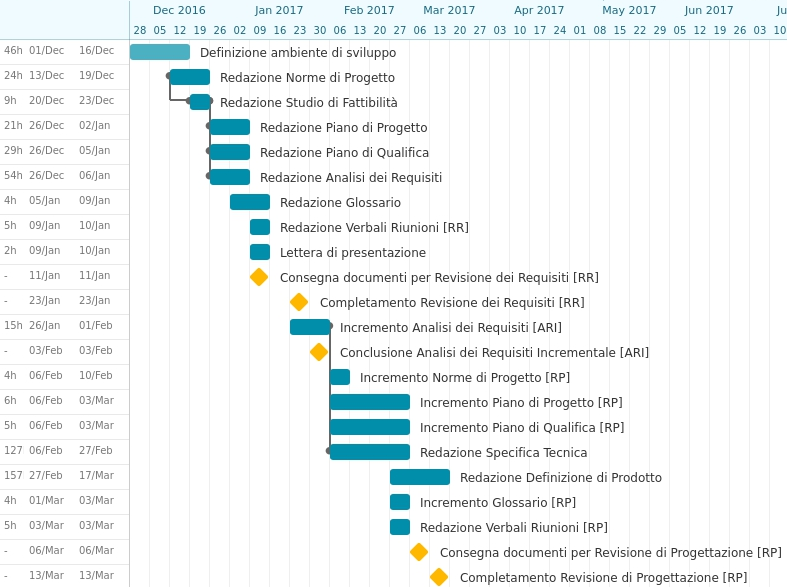
\includegraphics[width=1.2\textwidth]{img/ganttweeks1.png}}
\label{tab:genweeks}
\caption{\gloss{Diagramma di Gantt} della pianificazione generale, in settimane (parte 1)}

Nota: la "dipendenza all'indietro" che sembra esistere tra \emph{Redazione Norme di Progetto} e \emph{Redazione Studio di Fattibilità} non esiste (vedi prossimi diagrammi in giorni).
\end{figure}


\begin{figure}[H]
\makebox[\textwidth][c]{
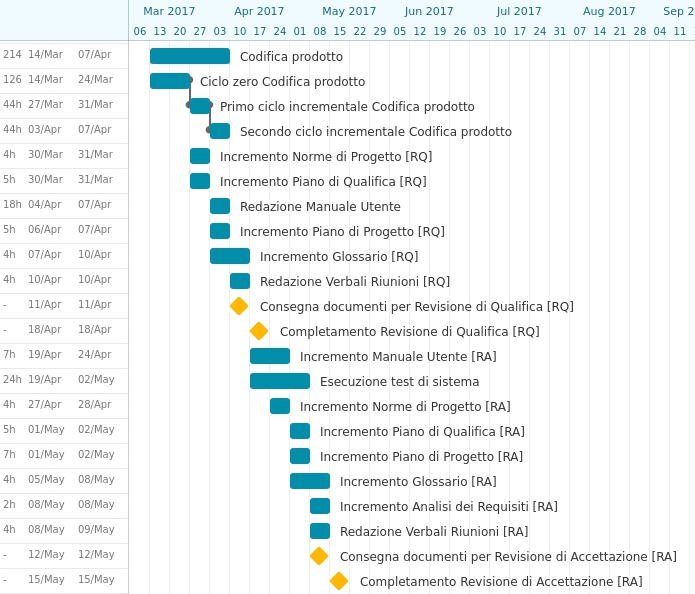
\includegraphics[width=1.2\textwidth]{img/ganttweeks2.png}}
\label{tab:genweeks}
\caption{\gloss{Diagramma di Gantt} della pianificazione generale, in settimane (parte 2)}
\end{figure}




\subsection{Suddivisione delle Attività}
	\subsubsection{\AR} \label{sec:AR}
	\textbf{Periodo}: dal 29-11-2016 al 11-01-2017.
	\\ Questo periodo inizia successivamente alla formazione del gruppo e finisce in corrispondenza della consegna dei documenti per la \emph{Revisione dei Requisiti}.
	Questo periodo prevede che siano stilati i seguenti documenti:
	\begin{description}
		\item[Norme di Progetto] in questo documento sono inserite tutte le norme che il \gloss{team} dovrà seguire e rispettare durante l'intero svolgimento delle attività. Tale documento è redatto dall'\AMx{}, mentre il \Vx{} ha il compito di certificare che tali norme siano state rispettate da tutto il gruppo;
		\item[Studio di Fattibilità] in questo documento sono analizzati i vari capitolati proposti. Per ogni capitolato, è stato analizzato il dominio applicativo/tecnologico e sono state inserite delle considerazioni in merito agli aspetti positivi e negativi;
		\item[Analisi dei requisiti] in questo documento sono raccolti tutti i requisiti progettuali necessari per comprendere più approfonditamente	il capitolato scelto con lo \emph{Studio di Fattibilità};
		\item[Piano di Progetto] questo documento è redatto dal \emph{Responsibile di Progetto} che organizza tutte le attività e stima le risorse, costi e tempi necessari per lo svolgimento del progetto;
		\item[Piano di Qualifica] questo documento è redatto dal \Vx{} che individua tutte le strategie di verifica e validazione che il \gloss{team} deve adottare per il progetto per ottenere e consegnare un prodotto di qualità;
		\item[Glossario] questo documento è steso da tutti i redattori in parallelo alla stesura degli altri documenti; esso contiene la spiegazione di alcuni termini presenti nei vari documenti al fine di chiarire il significato del termine stesso;
		\item[Lettera di presentazione] questo documento viene presentato al committente al fine di mostrare l'interesse del gruppo di partecipare alla gara d'appalto.
	\end{description}
	
	

\begin{figure}[H]
\makebox[\textwidth][c]{
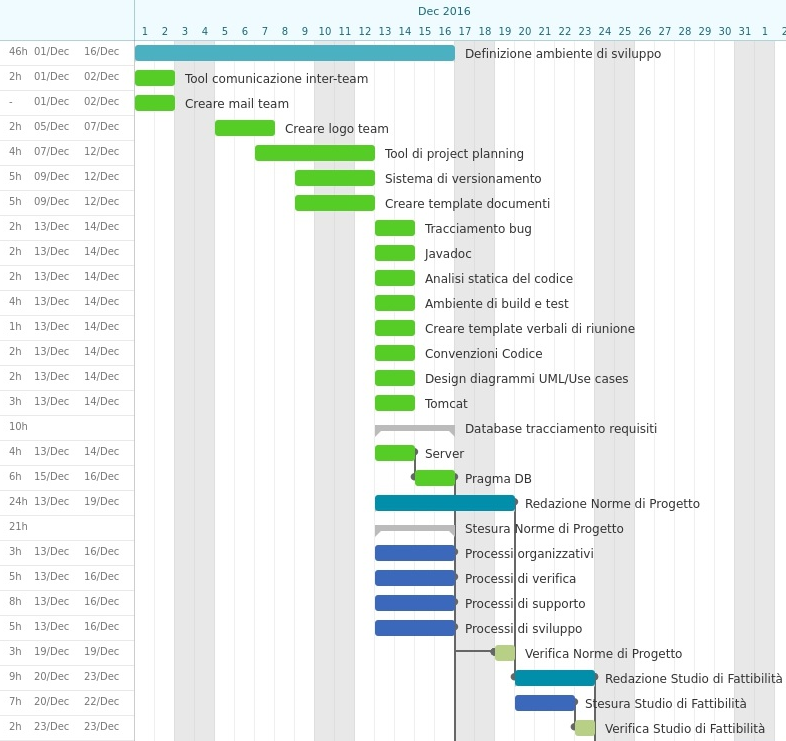
\includegraphics[width=1.2\textwidth]{img/ganttan1.png}}
\label{img:genweeks1}
\caption{\gloss{Diagramma di Gantt} della pianificazione della fase di \AR, in giorni (parte 1)}
\end{figure}


\begin{figure}[H]
\makebox[\textwidth][c]{
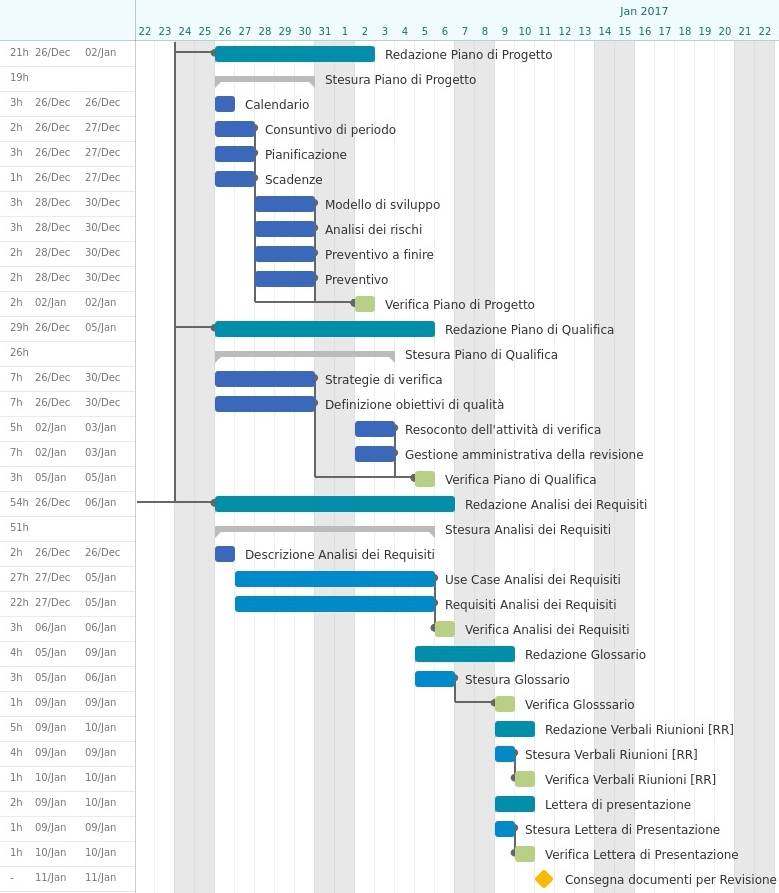
\includegraphics[width=1.2\textwidth]{img/ganttan2.png}}
\label{tab:genweeks2}
\caption{\gloss{Diagramma di Gantt} della pianificazione della fase di \AR, in giorni (parte 2)}

Note:
\begin{itemize}
\item l'attività \emph{Redazione Analisi dei Requisiti} ha una dipendenza verso l'attività \gloss{PragmaDB} appartenente all'attività \emph{Database tracciamento requisiti};
\item le attività \emph{Redazione Piano di Progetto}, \emph{Redazione Piano di Qualifica} e \emph{Redazione Analisi dei Requisiti} hanno una dipendenza verso l'attività \emph{Redazione Studio di Fattibilità}.
\end{itemize} 
\end{figure}
		
	\subsubsection{\ARI} \label{sec:ARI}
	\textbf{Periodo}: dal 24-01-2017 al 03-02-2017.
	\\ Questo periodo inizia in concomitanza con la \emph{Revisione dei Requisiti} e termina con una \gloss{milestone} interna che corrisponde all'inizio della \PA. In questo periodo, il gruppo mira ad integrare la documentazione precedentemente prodotta (in modo particolare l'\AR), con le correzioni suggerite durante la \emph{Revisione dei Requisiti} ed ampliarla tramite la definizione di alcuni requisiti opzionali.



\begin{figure}[H]
\makebox[\textwidth][c]{
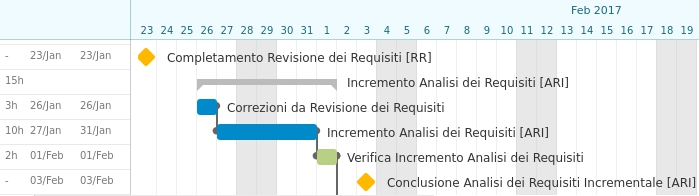
\includegraphics[width=1.2\textwidth]{img/ganttari.png}}
\label{tab:genweeks}
\caption{\gloss{Diagramma di Gantt} della pianificazione della fase di \ARI, in giorni}
\end{figure}

	
	\subsubsection{\PA} \label{sec:PA}
	\textbf{Periodo}: dal 06-02-2017 al 06-03-2017.	
	\\ Questo periodo inizia subito dopo \ARI{} e si conclude con la consegna dei documenti per la \emph{Revisione di Progettazione}. La \PA{} prevede la stesura della progettazione ad alto livello e prevede lo svolgimento delle seguenti attività:
	\begin{description}
		\item[Incremento dei Documenti] in questa attività sono incrementati tutti i documenti della \PA{};
		\item[Redazione Specifica Tecnica] in questa attività sono descritte nel documento le scelte progettuali ad alto livello che il prodotto dovrà rispettare.
	\end{description}
	

\begin{figure}[H]
\makebox[\textwidth][c]{
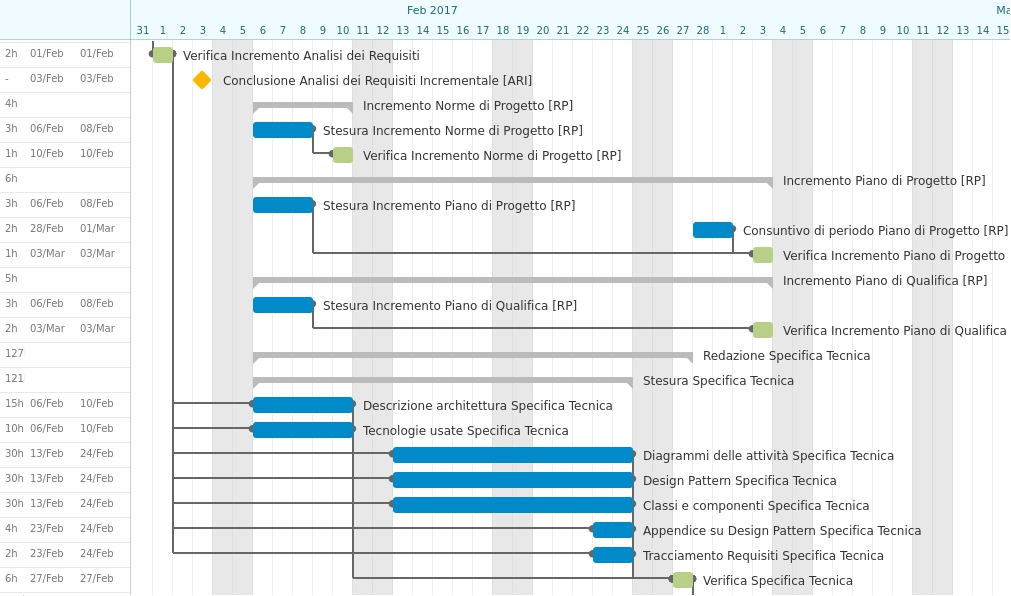
\includegraphics[width=1.2\textwidth]{img/ganttpa1.png}}
\label{tab:ganttpa1}
\caption{\gloss{Diagramma di Gantt} della pianificazione della fase di \PA, in giorni (parte 1)}
\end{figure}

\begin{figure}[H]
\makebox[\textwidth][c]{
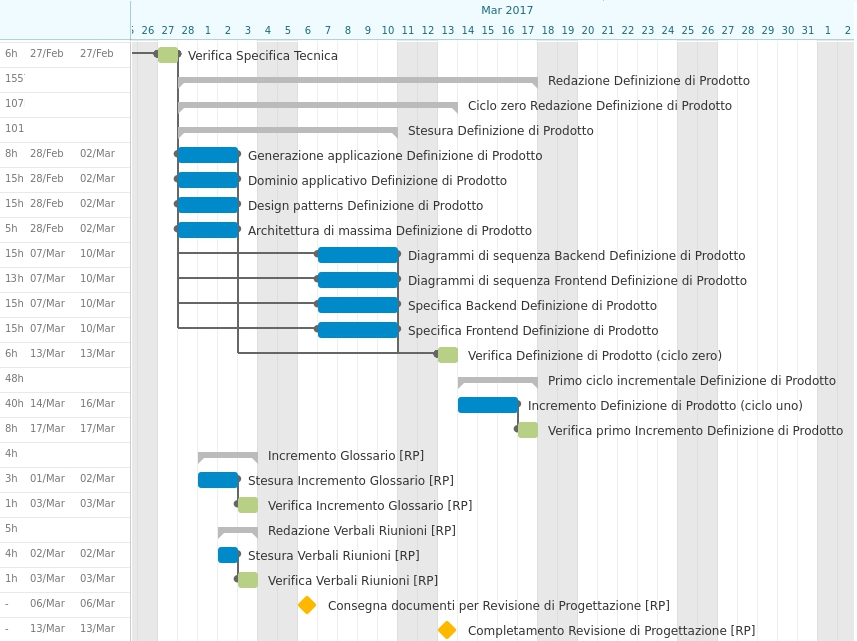
\includegraphics[width=1.2\textwidth]{img/ganttpa2.png}}
\label{tab:ganttpa2}
\caption{\gloss{Diagramma di Gantt} della pianificazione della fase di \PA, in giorni (parte 2)}

Note:
\begin{itemize}
\item Per raggiungere il completamento della fase successiva in tempo per la \emph{Revisione di Qualifica} si prevede di usare parte del tempo prima della scadenza del 06-03-2017 per la stesura della \emph{Definizione di Prodotto}.
\end{itemize} 
\end{figure}


	\subsubsection{\PDC} \label{sec:PDC}
	\textbf{Periodo}: dal 06-03-2017 al 11-04-2017.	
	\\ Questo periodo inizia subito dopo la \PA{} e si conclude con la consegna dei documenti per la \emph{Revisione di Qualifica}. La \PDC{} prevede la stesura della \emph{Definizione di Prodotto} e successivamente sarà avviata la fase di codifica. Le attività da svolgere sono le seguenti:
	\begin{description}
		\item[Incremento dei Documenti] in questa attività sono incrementati tutti i documenti basandosi sui risultati della \emph{Revisione di Progettazione}; 
		\item[Definizione di Prodotto] in questa attività è stilato questo documento che contiene la struttura e la relazione tra i vari componenti del prodotto, in base a quanto riportato nel documento \emph{Specifica Tecnica};
		\item[Codifica] in questa attività si procede allo sviluppo del codice del software da parte dei \emph{Programmatori}, attenendosi a quanto è riportato nella \emph{Definizione di Prodotto}; 
		\item[Redazione Manuale Utente] in questa attività si crea il documento destinato all'utente finale, che ha lo scopo di fornire le linee guida per il corretto utilizzo del software. Inoltre si crea il manuale utente sviluppatore, mirato a chiunque desideri ampliare il software già esistente.
	\end{description}
	
\begin{figure}[H]
\makebox[\textwidth][c]{
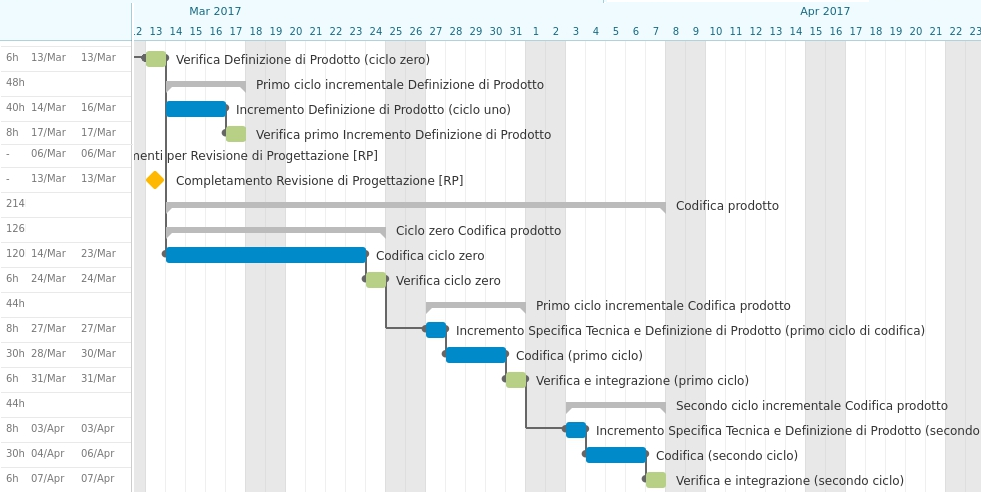
\includegraphics[width=1.2\textwidth]{img/ganttpdc1.png}}
\label{tab:ganttpa1}
\caption{\gloss{Diagramma di Gantt} della pianificazione della fase di \PDC, in giorni (parte 1)}
\end{figure}

\begin{figure}[H]
\makebox[\textwidth][c]{
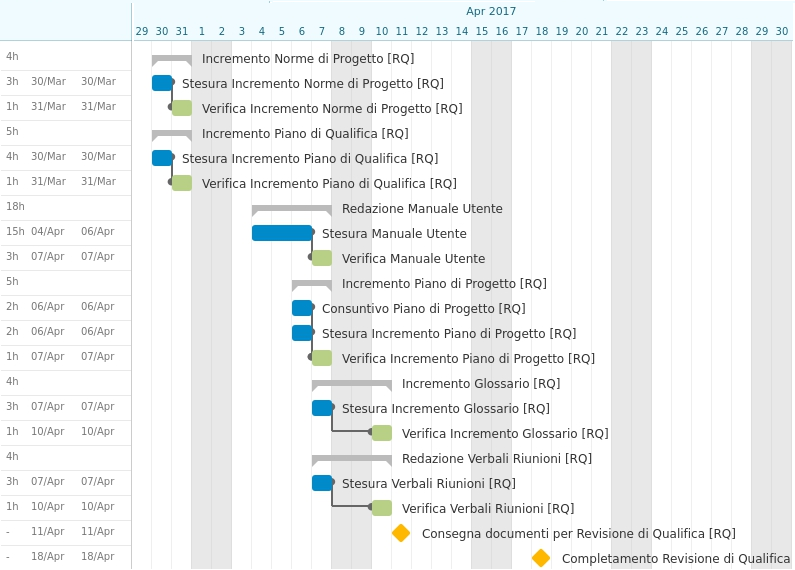
\includegraphics[width=1.2\textwidth]{img/ganttpdc2.png}}
\label{tab:ganttpa1}
\caption{\gloss{Diagramma di Gantt} della pianificazione della fase di \PDC, in giorni (parte 2)}
\end{figure}


	\subsubsection{Verifica e Validazione} \label{sec:VV}

	\subsubsection{\VV} \label{sec:VV}
	\textbf{Periodo}: dal 18-04-2017 al 14-05-2017.
	\\ Questo periodo inizia subito dopo la \PDC{} e si conclude con la consegna del prodotto finale alla \emph{Revisione di Accettazione}. In questo periodo vengono effettuati i test del software, atti a garantire un prodotto finale che soddisfi i requisiti contenuti nell'\AR. Le attività da svolgere sono:
	\begin{description}
		\item[Test] effettuare dei test per il collaudo del sistema;
		\item[Incremento e Verifica dei Documenti] in questa attività verranno incrementati verificati tutti i documenti, basandosi sui risultati della \emph{Revisione di Qualifica}.
	\end{description}		
	
\begin{figure}[H]
\makebox[\textwidth][c]{
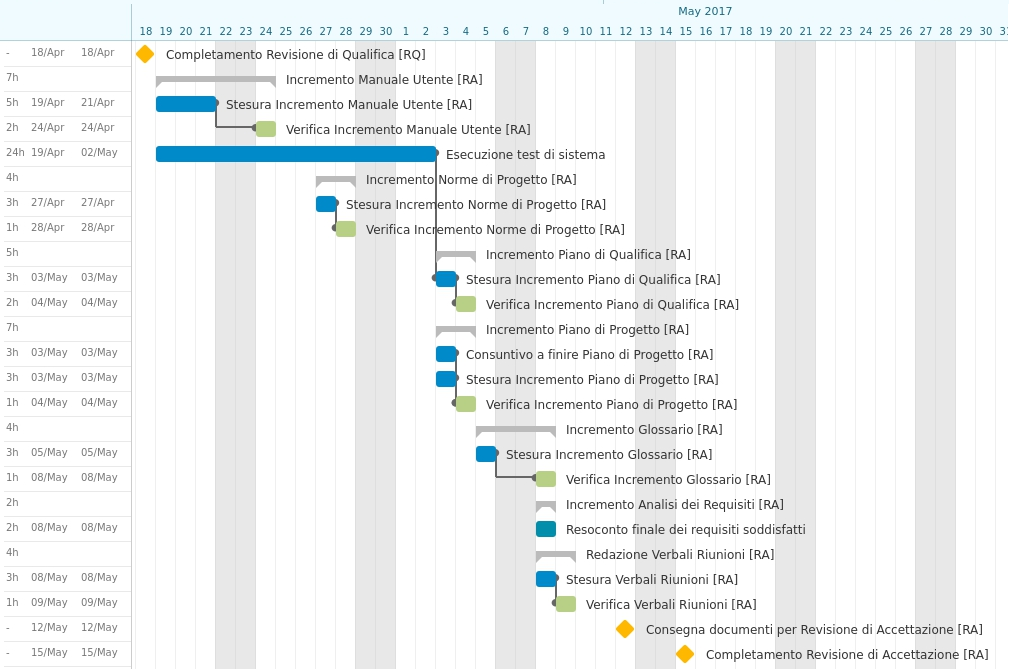
\includegraphics[width=1.2\textwidth]{img/ganttva.png}}
\label{tab:ganttpa1}
\caption{\gloss{Diagramma di Gantt} della pianificazione della fase di \VV, in giorni}
\end{figure}

\pagebreak
	
\section{Suddivisione delle ore lavorative e preventivo} \label{sec:preventivo}
Di seguito è riportata la pianificazione di dettaglio delle attività, suddivisa nei periodi descritti precedentemente. Per ogni periodo, sono presenti una tabella e dei grafici che descrivono e rappresentano i ruoli assunti da ciascun componente, il relativo quantitativo di ore impiegato e la rispettiva retribuzione.
A conclusione, è illustrato un quadro riassuntivo.


\newcommand{\roww}[7]{
	#1 & #2 & #3 & #4 & #5 & #6 & #7
}

\newcommand{\x}[7]{

\begin{figure}[h]
  \begin{tabular}{ | l | c | c | c | c | c | c | r   }
    \hline
    Ruolo / persona & \R & \AM & \AN & \PJ & \PG & \V & Totale ore per persona \\ \hline
    \PB & \roww[#1] \\ \hline
    \LB & \roww[#2] \\ \hline
    \GG & \roww[#3] \\ \hline
    \MM & \roww[#4] \\ \hline
    \LS & \roww[#5] \\ \hline
    \AZ & \roww[#6] \\ \hline
    Totale ore per ruolo & \roww[#7] \\ \hline
  \end{tabular}
\end{figure} 
}

\newcommand{\intropreventivo}[1]
{
Di seguito si riporta la divisione oraria pianificata nella fase di #1.

Successivamente sono evidenziate graficamente la divisione delle ore per persona e per ruolo. 
}


\newcommand{\introcosto}[1]
{
Di seguito si riporta il costo della #1.
}

\pagebreak[4]
\subsection{\AR}

\intropreventivo{\AR}
% i colori danno problemi di visualizzazione alle linee
\begin{figure}[H]
\makebox[\textwidth][c]
{
\definecolor{white2}{rgb}{0.95,0.95,0.95}
\definecolor{white3}{rgb}{0.9,0.9,0.9}
%\rowcolors{1}{white}{white2}

  \begin{tabular}{ | l | c | c | c | c | c | c | r |}
    \hline
    \rowcolor[gray]{.9}
    Ruolo / persona & \R & \AM & \AN & \PJ & \PG & \V & Tot ore/persona \\ \hline
    \PB & 7 & 3 & 14 & 0 & 0 & 7 & 31 \\ \hline
    \LB & 12 & 11 & 6 & 0 & 0 & 6 & 35 \\ \hline
    \GG & 0 & 24 & 8 & 0 & 0 & 3 & 35 \\ \hline
    \MM & 0 & 20 & 8 & 0 & 0 & 4 & 32\\ \hline
    \LS & 0 & 2 & 12 & 0 & 0 & 17 & 31\\ \hline
    \AZ & 1 & 4 & 13 & 0 & 0 & 12 & 30 \\ \hline
    \rowcolor[gray]{.9}

    Totale ore/ruolo & 20 & 64 & 61 & 0 & 0 & 49 & 194 \\ \hline
    
  \end{tabular}
}
\caption{Ore/ruolo per persona nella fase di \AR.}

%\vspace*{1 cm}
\end{figure}

\pagebreak


\begin{figure}[H]
\makebox[\textwidth][c]
{
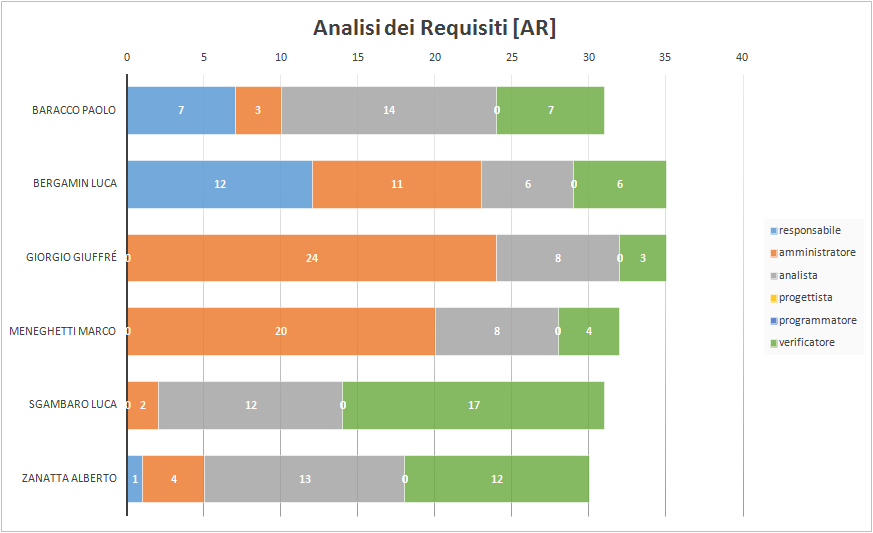
\includegraphics[width=1.1\textwidth]{img/orear1.png}
}
\caption{Ore/ruolo per persona nella fase di \AR.}
\label{fig:ar1}

\end{figure}

\begin{figure}[H]
\makebox[\textwidth][c]{
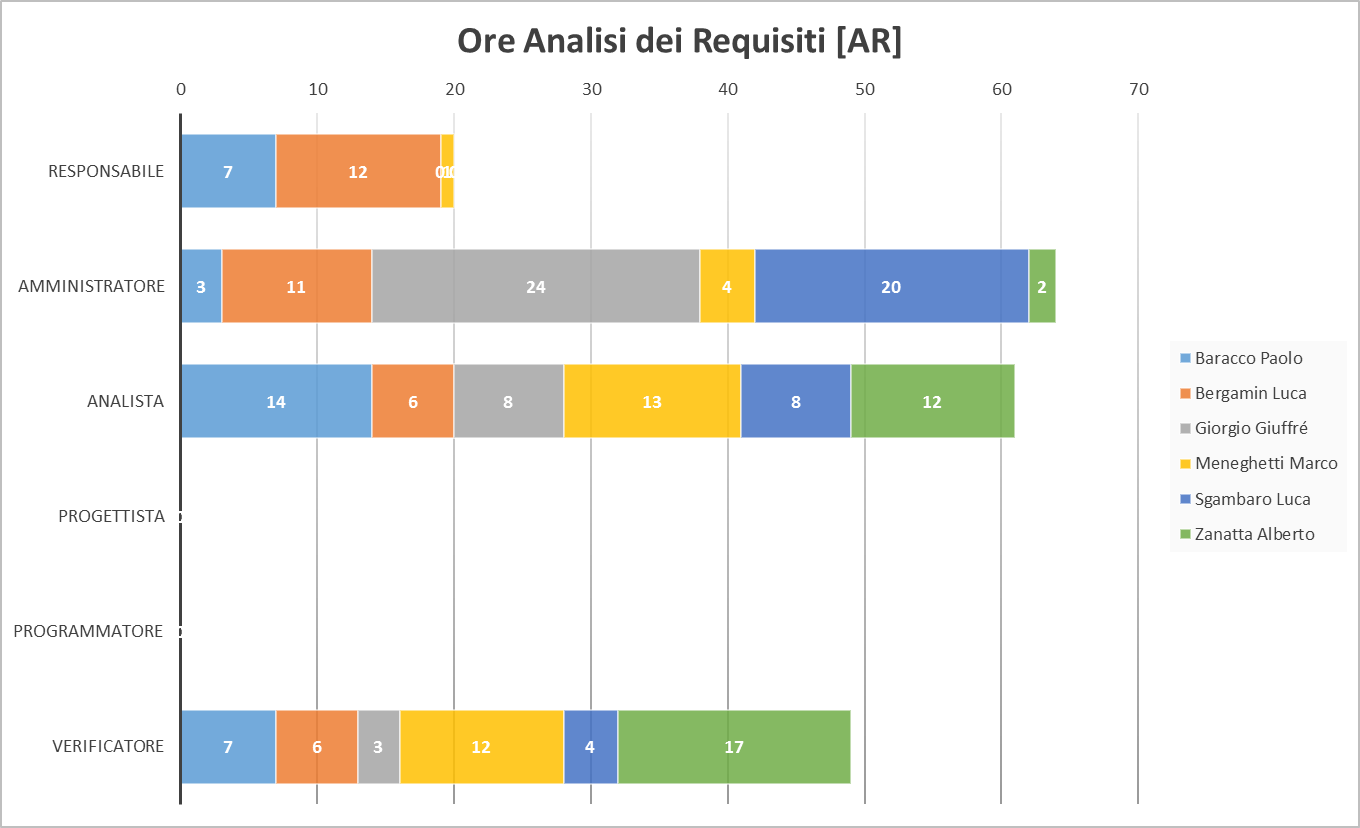
\includegraphics[width=1.1\textwidth]{img/orear2.png}\par
}
\caption{Ore/persona per ruolo nella fase di \AR.}
\label{fig:ar2}
\end{figure}
	
\pagebreak
\subsubsection{Costo \AR}
	
\introcosto{\AR}
Questo costo viene fornito a scopo informativo e rappresenta l'investimento effettuato da {\hx} prima dell'aggiudicazione dell'appalto e perciò tale periodo \textbf{non è a carico del cliente}. 

Gli sforzi maggiori si evidenziano nel ruolo di:
\begin{itemize}
\item {\AMx} a causa dell'impegno aggiuntivo dedicato alla creazione di un proprio \gloss{Way of Working};
\item {\ANx} per gli sforzi impiegati a raggiungere una comprensione profonda dei requisiti del progetto affrontato.
\end{itemize}

\begin{figure}[H]
\makebox[\textwidth][c]
{
\definecolor{white2}{rgb}{0.95,0.95,0.95}
\definecolor{white3}{rgb}{0.9,0.9,0.9}
%\rowcolors{1}{white}{white2}

  \begin{tabular}{ | l | c | c | c | c | c | c | r |}
    \hline
    \rowcolor[gray]{.9}
    Ruolo / persona & \R & \AM & \AN & \PJ & \PG & \V & Tot euro/persona \\ \hline
    \PB & 210 & 60 & 350 & 0 & 0 & 105 & 725 \\ \hline
    \LB & 360 & 220 & 150 & 0 & 0 & 90 & 820 \\ \hline
    \GG & 0 & 480 & 200 & 0 & 0 & 45 & 725 \\ \hline
    \MM & 0 & 400 & 200 & 0 & 0 & 60 & 660 \\ \hline
    \LS & 0 & 40 & 300 & 0 & 0 & 255 & 595 \\ \hline
    \AZ & 30 & 80 & 325 & 0 & 0 & 180 & 615 \\ \hline
    \rowcolor[gray]{.9}

    Totale euro/ruolo & 600 & 1280 & 1525 & 0 & 0 & 735 & 4140 \\ \hline
  \end{tabular}
  
}\label{tab:car}

  \caption{Tabella costo {\AR} per ruolo e per persona, valori in euro (\euro).}
\end{figure}

\begin{figure}[H]
\makebox[\textwidth][c]{
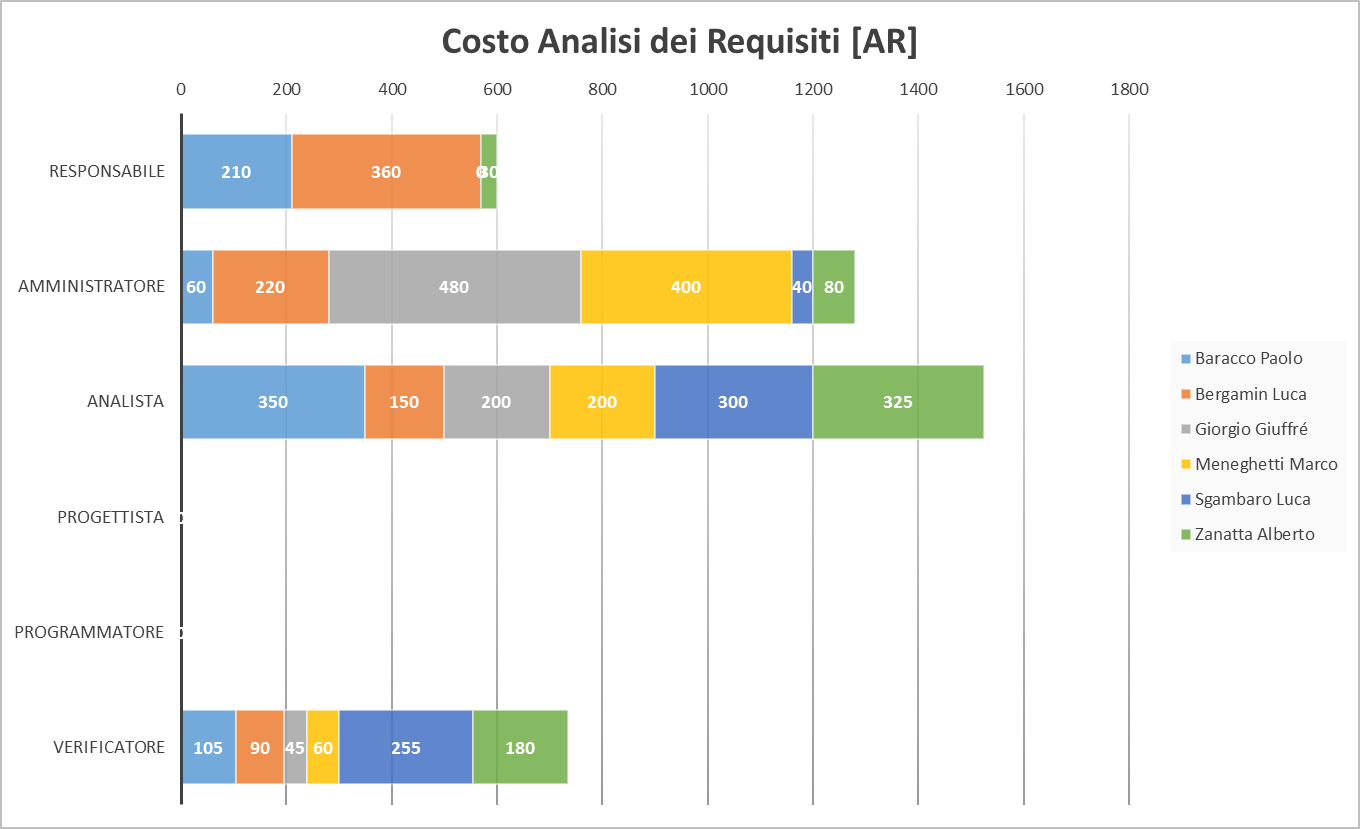
\includegraphics[width=1.05\textwidth]{img/costoar.png}\par
}
\caption{Costo {\AR} per ruolo, valori in euro (\euro).}
\label{fig:car}
\end{figure}



%\x
%{\roww{7}{3}{14}{0}{0}{7}{31}}
%{\roww{12}{11}{6}{0}{0}{6}{35}}
%{\roww{0}{24}{8}{0}{0}{3}{35}}
%{\roww{0}{20}{8}{0}{0}{4}{32}}
%{\roww{0}{2}{12}{0}{0}{17}{31}}
%{\roww{1}{4}{13}{0}{0}{12}{30}}
%{\roww{20}{64}{61}{0}{0}{49}{194}}


\pagebreak[4]
\subsection{\ARI}
\intropreventivo{\ARI}


\begin{figure}[H]

\makebox[\textwidth][c]
{
\definecolor{white2}{rgb}{0.95,0.95,0.95}
\definecolor{white3}{rgb}{0.9,0.9,0.9}
%\rowcolors{1}{white}{white2}

  \begin{tabular}{ | l | c | c | c | c | c | c | r |}
    \hline
    \rowcolor[gray]{.9}
    Ruolo / persona & \R & \AM & \AN & \PJ & \PG & \V & Tot ore/persona \\ \hline
    \PB & 0 & 0 & 0 & 0 & 0 & 0 & 0 \\ \hline
    \LB & 0 & 0 & 0 & 0 & 0 & 0 & 0 \\ \hline
    \GG & 0 & 0 & 0 & 0 & 0 & 2 & 2 \\ \hline
    \MM & 0 & 0 & 0 & 0 & 0 & 0 & 0 \\ \hline
    \LS & 0 & 0 & 5 & 0 & 0 & 0 & 5 \\ \hline
    \AZ & 0 & 0 & 8 & 0 & 0 & 0 & 8 \\ \hline
    \rowcolor[gray]{.9}

    Totale ore/ruolo & 0 & 0 & 13 & 0 & 0 & 2 & 15 \\ \hline
    
  \end{tabular}
}
\caption{Ore/ruolo per persona nella fase di \ARI.}

\end{figure} 
% i colori danno problemi di visualizzazione alle linee
\pagebreak


\begin{figure}[H]
\makebox[\textwidth][c]{
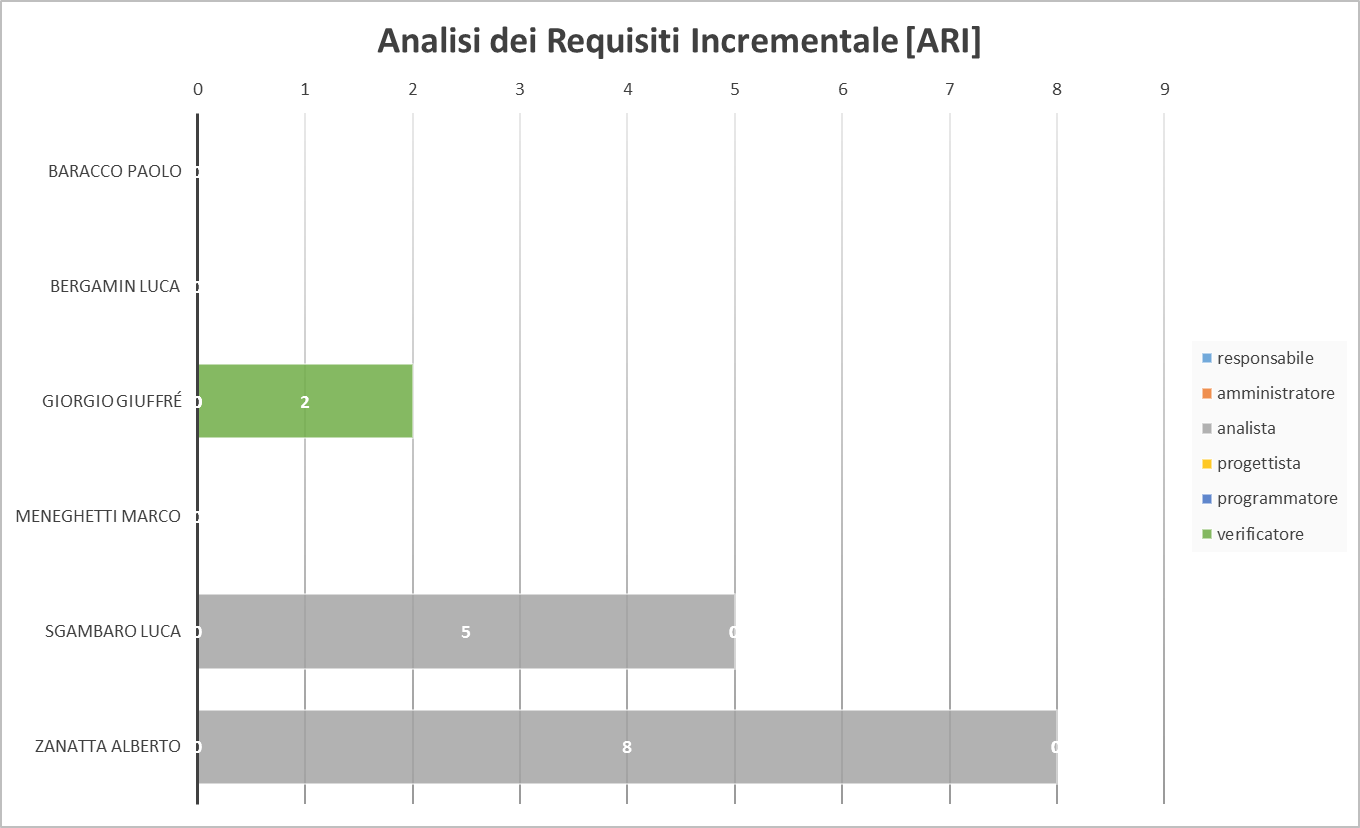
\includegraphics[width=1.15\textwidth]{img/oreari1.png}}
\caption{Ore/ruolo per persona nella fase di \ARI.}
\label{fig:ari}

\end{figure}

\begin{figure}[H]
\makebox[\textwidth][c]{
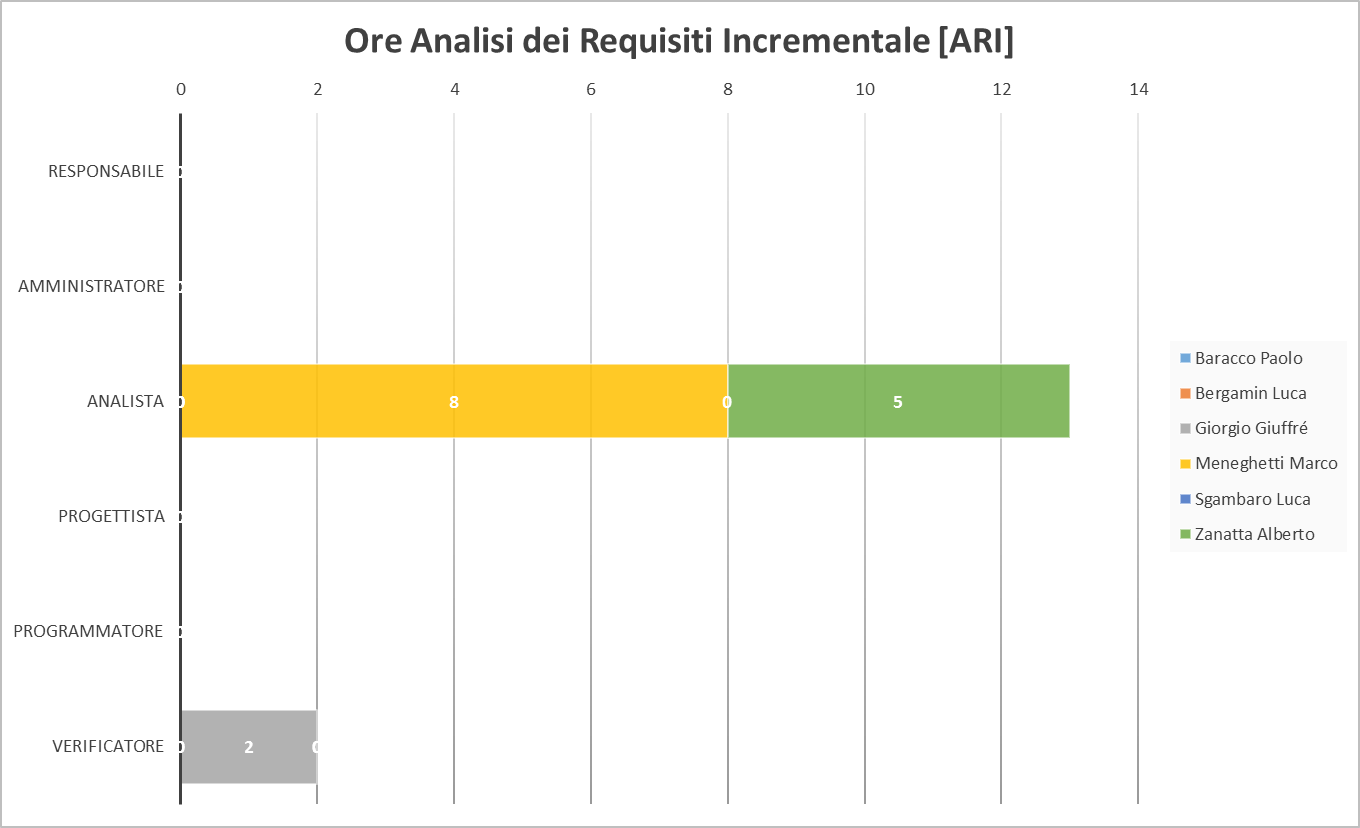
\includegraphics[width=1.15\textwidth]{img/oreari2.png}}
\caption{Ore/persona per ruolo nella fase di \ARI.}
\label{fig:ari2}

\end{figure}

\pagebreak

\subsubsection{Costo \ARI}

\introcosto{\ARI}
Questo costo rappresenta gli sforzi che {\hx} affronterà al fine di consolidare la comprensione dei requisiti del progetto.

Tale periodo è ridotto rispetto a quanto desiderato in quanto coincidente con la sessione d'esami dell'Università degli Studi di Padova. % togliere?

Gli sforzi maggiori si evidenziano nel ruolo di:
\begin{itemize}
\item {\ANx} per gli sforzi impiegati a raggiungere una comprensione profonda dei requisiti del progetto affrontato.
\end{itemize}

\begin{figure}[H]
\makebox[\textwidth][c]
{
\definecolor{white2}{rgb}{0.95,0.95,0.95}
\definecolor{white3}{rgb}{0.9,0.9,0.9}
%\rowcolors{1}{white}{white2}

  \begin{tabular}{ | l | c | c | c | c | c | c | r |}
    \hline
    \rowcolor[gray]{.9}
    Ruolo / persona & \R & \AM & \AN & \PJ & \PG & \V & Tot euro/persona \\ \hline
    \PB & 0 & 0 & 0 & 0 & 0 & 0 & 0 \\ \hline
    \LB & 0 & 0 & 0 & 0 & 0 & 0 & 0 \\ \hline
    \GG & 0 & 0 & 0 & 0 & 0 & 30 & 30 \\ \hline
    \MM & 0 & 0 & 125 & 0 & 0 & 0 & 0 \\ \hline
    \LS & 0 & 0 & 200 & 0 & 0 & 0 & 125 \\ \hline
    \AZ & 0 & 0 & 325 & 0 & 0 & 30 & 200 \\ \hline
    \rowcolor[gray]{.9}

    Totale euro/ruolo & 0 & 0 & 325 & 0 & 0 & 30 & 355 \\ \hline
  \end{tabular}
  
}\label{tab:cari}

  \caption{Tabella costo {\ARI} per ruolo e per persona, valori in euro (\euro).}
\end{figure}

\begin{figure}[H]
\makebox[\textwidth][c]{
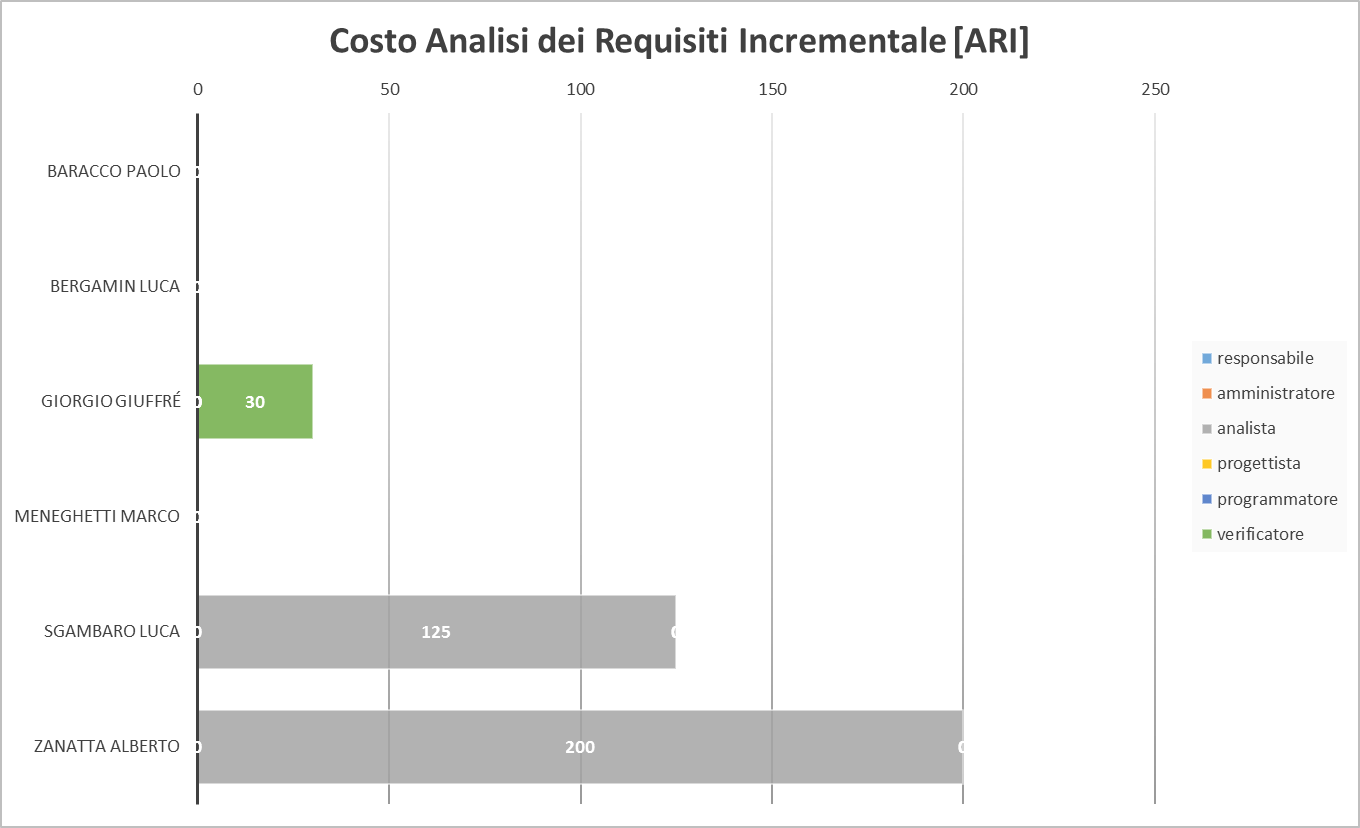
\includegraphics[width=1.2\textwidth]{img/costoari.png}
}
\caption{Costo {\ARI} per ruolo, valori in euro (\euro).}


\end{figure}

\pagebreak[4]

\subsection{\PA}
\intropreventivo{\PA}

\begin{figure}[H]
\definecolor{white2}{rgb}{0.95,0.95,0.95}
\definecolor{white3}{rgb}{0.9,0.9,0.9}
%\rowcolors{1}{white}{white2}

\makebox[\textwidth][c]
{
  \begin{tabular}{ | l | c | c | c | c | c | c | r |}
    \hline
    \rowcolor[gray]{.9}
    Ruolo / persona & \R & \AM & \AN & \PJ & \PG & \V & Tot ore/persona \\ \hline
    \PB & 0 & 0 & 0 & 30 & 0 & 6 & 36 \\ \hline
    \LB & 0 & 3 & 0 & 38 & 0 & 1 & 42 \\ \hline
    \GG & 3 & 0 & 0 & 35 & 0 & 1 & 39 \\ \hline
    \MM & 0 & 0 & 0 & 45 & 0 & 4 & 49 \\ \hline
    \LS & 2 & 0 & 0 & 40 & 0 & 6 & 48 \\ \hline
    \AZ & 0 & 3 & 0 & 36 & 0 & 4 & 40 \\ \hline
    \rowcolor[gray]{.9}

    Totale ore/ruolo & 5 & 3 & 0 & 224 & 0 & 22 & 254 \\ \hline
    
  \end{tabular}
}
\caption{Ore/ruolo per persona nella fase di \PA.}
\end{figure} 
% i colori danno problemi di visualizzazione alle linee
\pagebreak

\begin{figure}[H]
\makebox[\textwidth][c]{
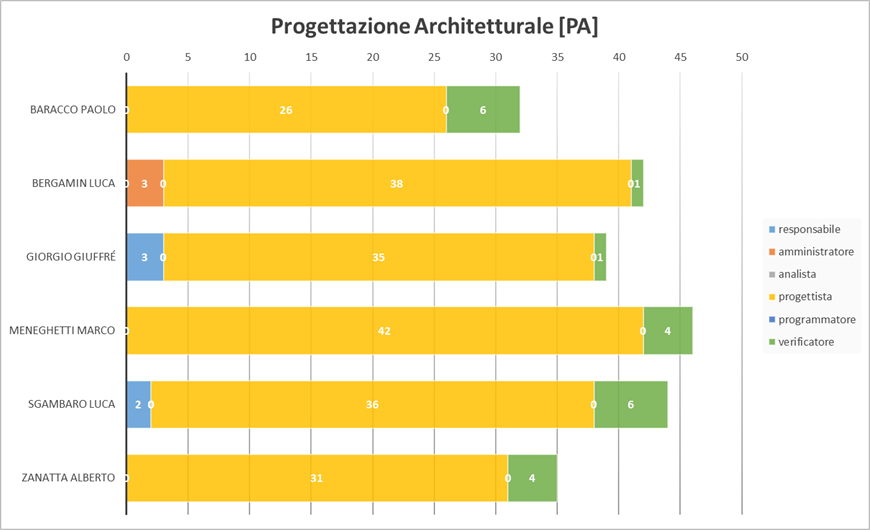
\includegraphics[width=1.1\textwidth]{img/orepa1.png}}
\caption{Ore/ruolo per persona nella fase di \PA.}
\label{fig:pa1}

\end{figure}

\begin{figure}[H]
\makebox[\textwidth][c]{
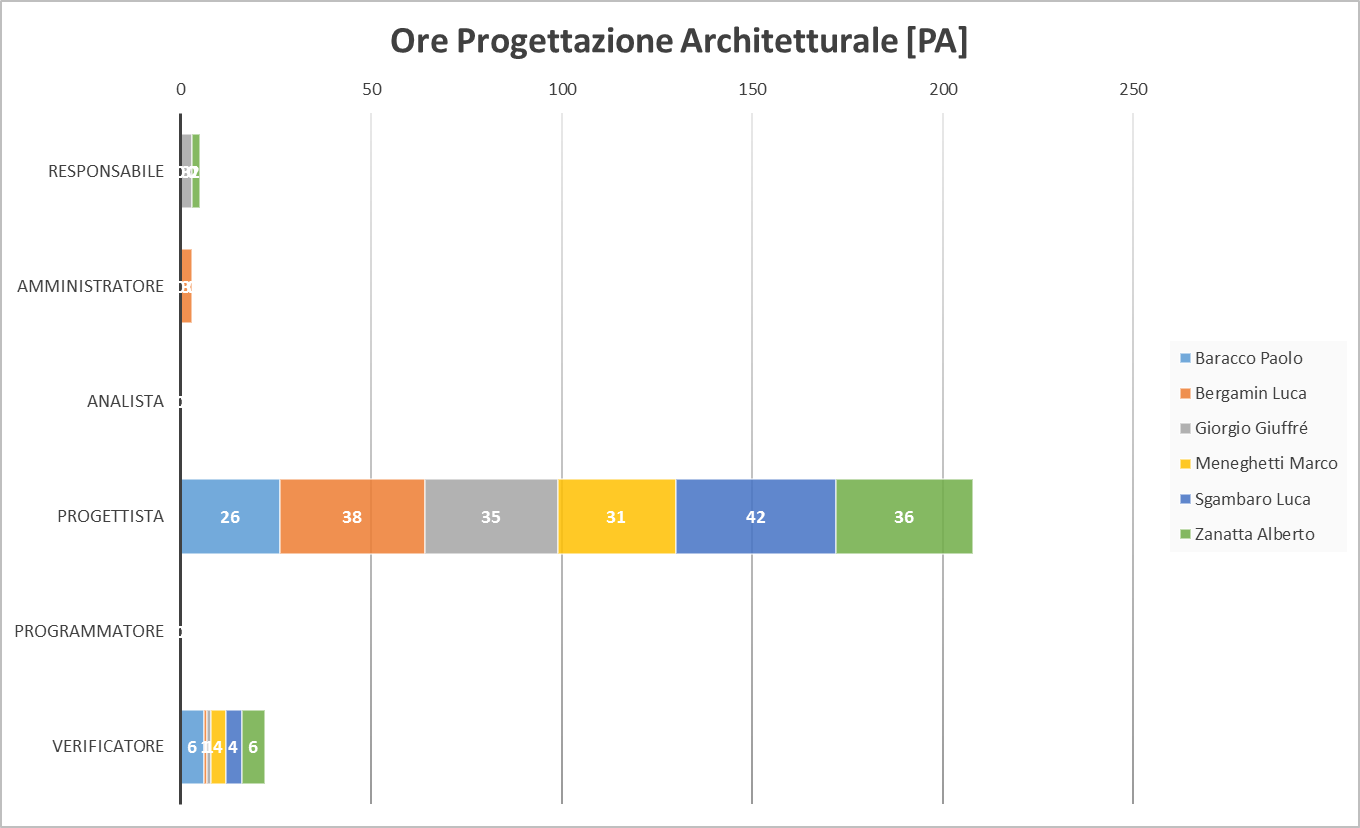
\includegraphics[width=1.1\textwidth]{img/orepa2.png}}
\caption{Ore/persona per ruolo nella fase di \PA.}
\label{fig:pa2}

\end{figure}

\pagebreak
\subsubsection{Costo \PA}
\introcosto{\PA}
Questa fase mira a consolidare la creazione di una solida base architetturale per \proj.

Gli sforzi maggiori si evidenziano nel ruolo di:
\begin{itemize}
\item {\PJx} per la creazione del documento di \emph{Specifica Tecnica} e parte del primo incremento della \emph{Definizione di Prodotto}.
\end{itemize}

\begin{figure}[H]
\makebox[\textwidth][c]
{
\definecolor{white2}{rgb}{0.95,0.95,0.95}
\definecolor{white3}{rgb}{0.9,0.9,0.9}
%\rowcolors{1}{white}{white2}

  \begin{tabular}{ | l | c | c | c | c | c | c | r |}
    \hline
    \rowcolor[gray]{.9}
    Ruolo / persona & \R & \AM & \AN & \PJ & \PG & \V & Tot euro/persona \\ \hline
    \PB & 0 & 0 & 0 & 660 & 0 & 90 & 750 \\ \hline
    \LB & 0 & 60 & 0 & 836 & 0 & 15 & 911 \\ \hline
    \GG & 90 & 0 & 0 & 770 & 0 & 15 & 875 \\ \hline
    \MM & 0 & 0 & 0 & 0 & 990 & 60 & 1050 \\ \hline
    \LS & 60 & 0 & 0 & 0 & 880 & 90 & 1030 \\ \hline
    \AZ & 0 & 0 & 0 & 0 & 792 & 60 & 852 \\ \hline
    \rowcolor[gray]{.9}

    Totale euro/ruolo & 150 & 60 & 0 & 4928 & 0 & 330 & 5468 \\ \hline
    
  \end{tabular}
  
}\label{tab:cpa}

  \caption{Tabella costo {\PA} per ruolo e per persona, valori in euro (\euro).}
\end{figure}

\begin{figure}[H]
\makebox[\textwidth][c]{
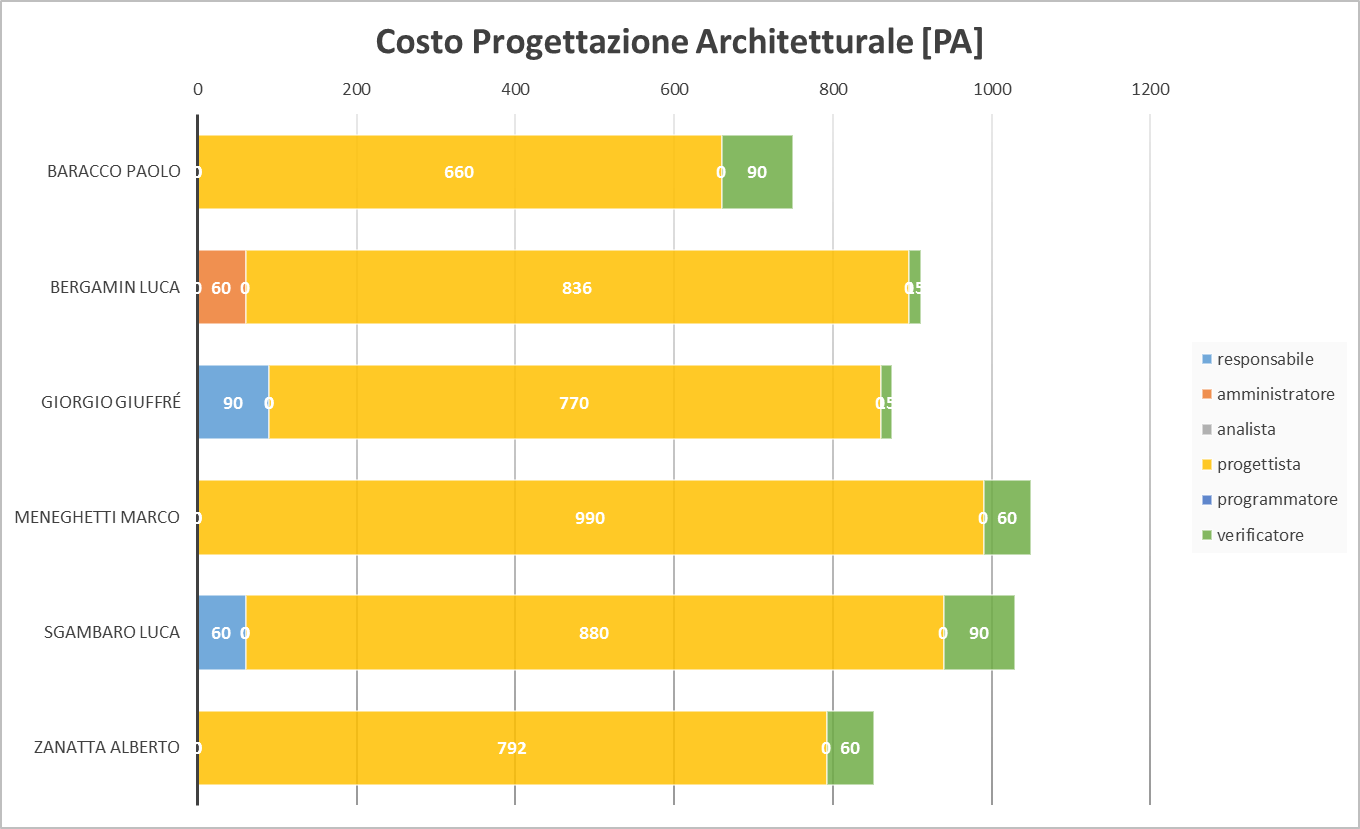
\includegraphics[width=1.2\textwidth]{img/costopa.png}}
  \caption{Costo \PA{} per ruolo e per persona, valori in euro (\euro).}
\end{figure}

\pagebreak[4]
\subsection{\PDC}
\intropreventivo{\PDC}

\begin{figure}[H]
\definecolor{white2}{rgb}{0.95,0.95,0.95}
\definecolor{white3}{rgb}{0.9,0.9,0.9}
%\rowcolors{1}{white}{white2}

\makebox[\textwidth][c]
{
  \begin{tabular}{ | l | c | c | c | c | c | c | r |}
    \hline
    \rowcolor[gray]{.9}
    Ruolo / persona & \R & \AM & \AN & \PJ & \PG & \V & Tot ore/persona \\ \hline
    \PB & 0 & 0 & 0 & 18 & 30 & 7 & 55 \\ \hline
    \LB & 0 & 5 & 0 & 8 & 30 & 13 & 56 \\ \hline
    \GG & 0 & 5 & 0 & 10 & 30 & 3 & 48 \\ \hline
    \MM & 2 & 0 & 0 & 0 & 30 & 8 & 40 \\ \hline
    \LS & 0 & 3 & 0 & 10 & 30 & 9 & 52 \\ \hline
    \AZ & 2 & 5 & 0 & 10 & 30 & 10 & 57 \\ \hline
    \rowcolor[gray]{.9}

    Totale ore/ruolo & 4 & 18 & 0 & 56 & 180 & 50 & 308 \\ \hline
    
  \end{tabular}
  }
    \caption{Ore/ruolo per persona nella fase di \PDC.}

\end{figure} 
% i colori danno problemi di visualizzazione alle linee

\pagebreak[4]

% USARE QUESTO PER IMMAGINI
\begin{figure}[H]
  \makebox[\textwidth][c]{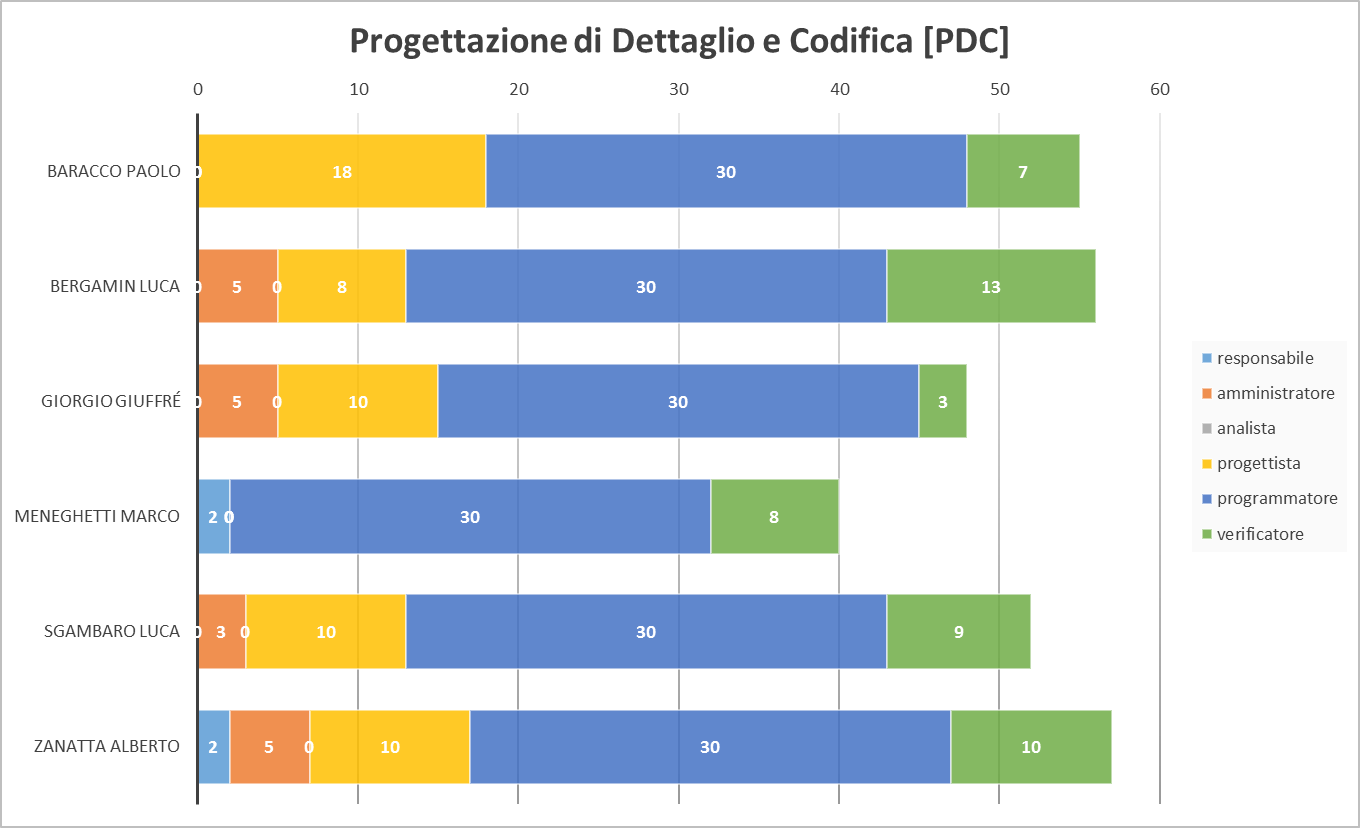
\includegraphics[width=1.1\textwidth]{img/orepdc1.png}}
  \caption{Ore/ruolo per persona nella fase di \PDC.}
\label{fig:pdc1}

\end{figure}



%	{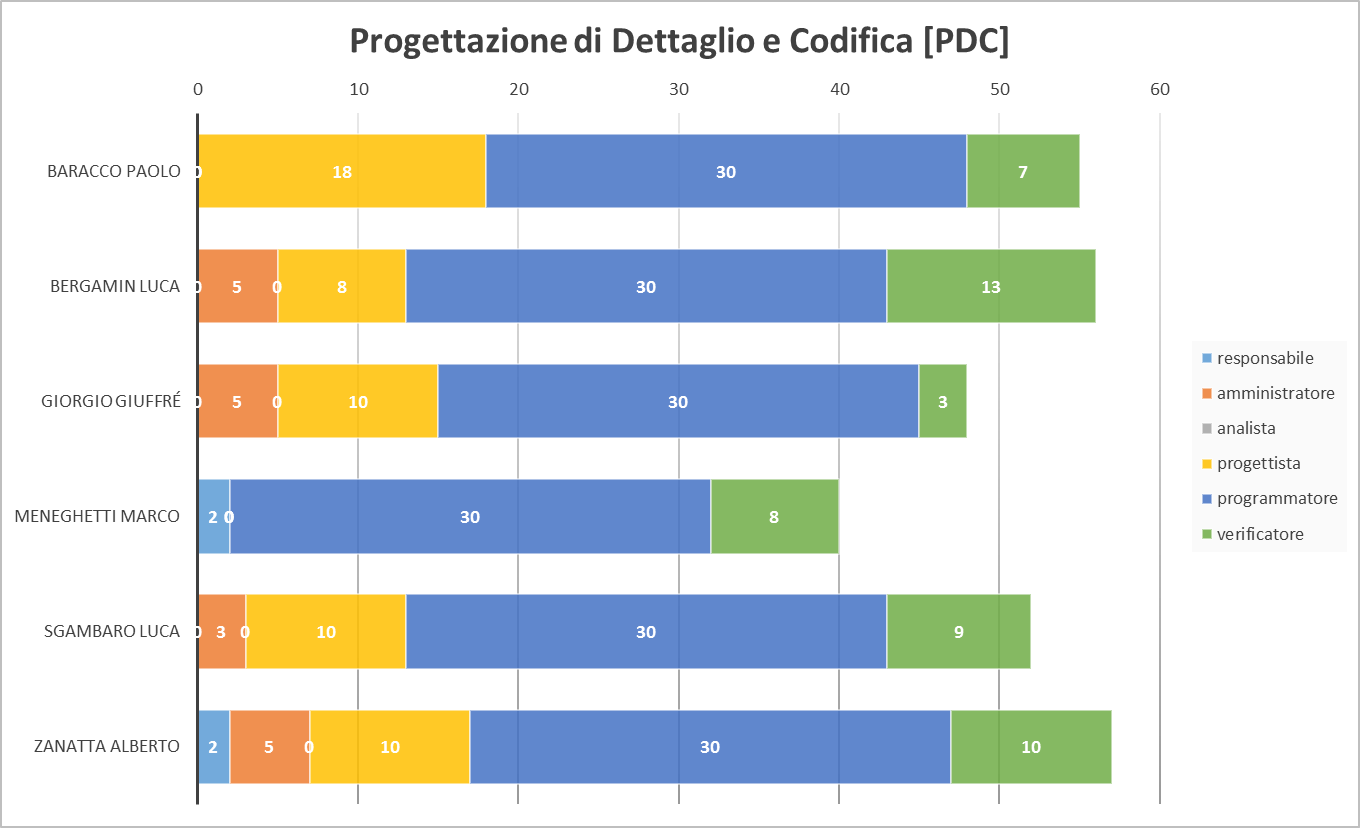
\includegraphics[width=15cm]{img/orepdc1.png}\par}

\begin{figure}[H]
\makebox[\textwidth][c]{
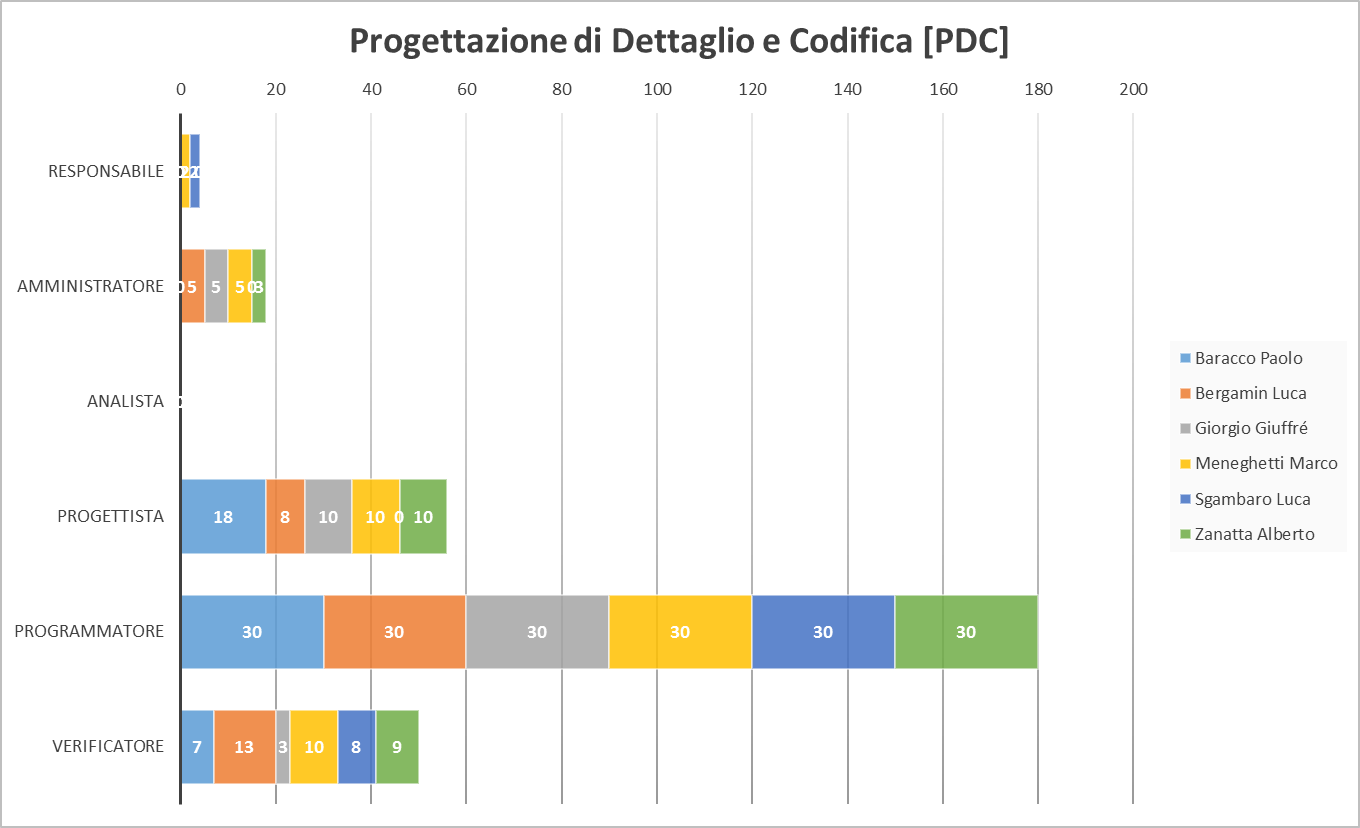
\includegraphics[width=1.1\textwidth]{img/orepdc2.png}}
\caption{Ore/persona per ruolo nella fase di \PDC.}
\label{fig:pdc2}

\end{figure}

\pagebreak
\subsubsection{Costo \PDC}
\introcosto{\PDC}
Questa fase mira a completare la \emph{Definizione di Prodotto} tramite incrementi e completare l'attività di codifica.

Gli sforzi maggiori si evidenziano nel ruolo di:
\begin{itemize}
\item {\PJx} per l'incremento della \emph{Definizione di Prodotto};
\item {\PGx} per l'attività di codifica;
\item {\Vx} per il controllo e la verifica del codice e dei documenti prodotti.
\end{itemize}

\begin{figure}[H]
\makebox[\textwidth][c]
{
\definecolor{white2}{rgb}{0.95,0.95,0.95}
\definecolor{white3}{rgb}{0.9,0.9,0.9}
%\rowcolors{1}{white}{white2}

  \begin{tabular}{ | l | c | c | c | c | c | c | r |}
    \hline
    \rowcolor[gray]{.9}
    Ruolo / persona & \R & \AM & \AN & \PJ & \PG & \V & Tot euro/persona \\ \hline
    \PB & 0 & 0 & 0 & 396 & 450 & 105 & 951 \\ \hline
    \LB & 0 & 100 & 0 & 176 & 450 & 195 & 921 \\ \hline
    \GG & 0 & 100 & 0 & 220 & 450 & 45 & 815 \\ \hline
    \MM & 60 & 0 & 0 & 0 & 450 & 120 & 630 \\ \hline
    \LS & 0 & 60 & 0 & 220 & 450 & 150 & 980 \\ \hline
    \AZ & 60 & 100 & 0 & 220 & 450 & 150 & 980 \\ \hline
    \rowcolor[gray]{.9}

    Totale euro/ruolo & 120 & 360 & 0 & 1232 & 2700 & 750 & 5162 \\ \hline
  \end{tabular}
  
}\label{tab:cpdc}

  \caption{Tabella costo {\PDC} per ruolo e per persona, valori in euro (\euro).}
\end{figure}
\begin{figure}[H]
\makebox[\textwidth][c]{
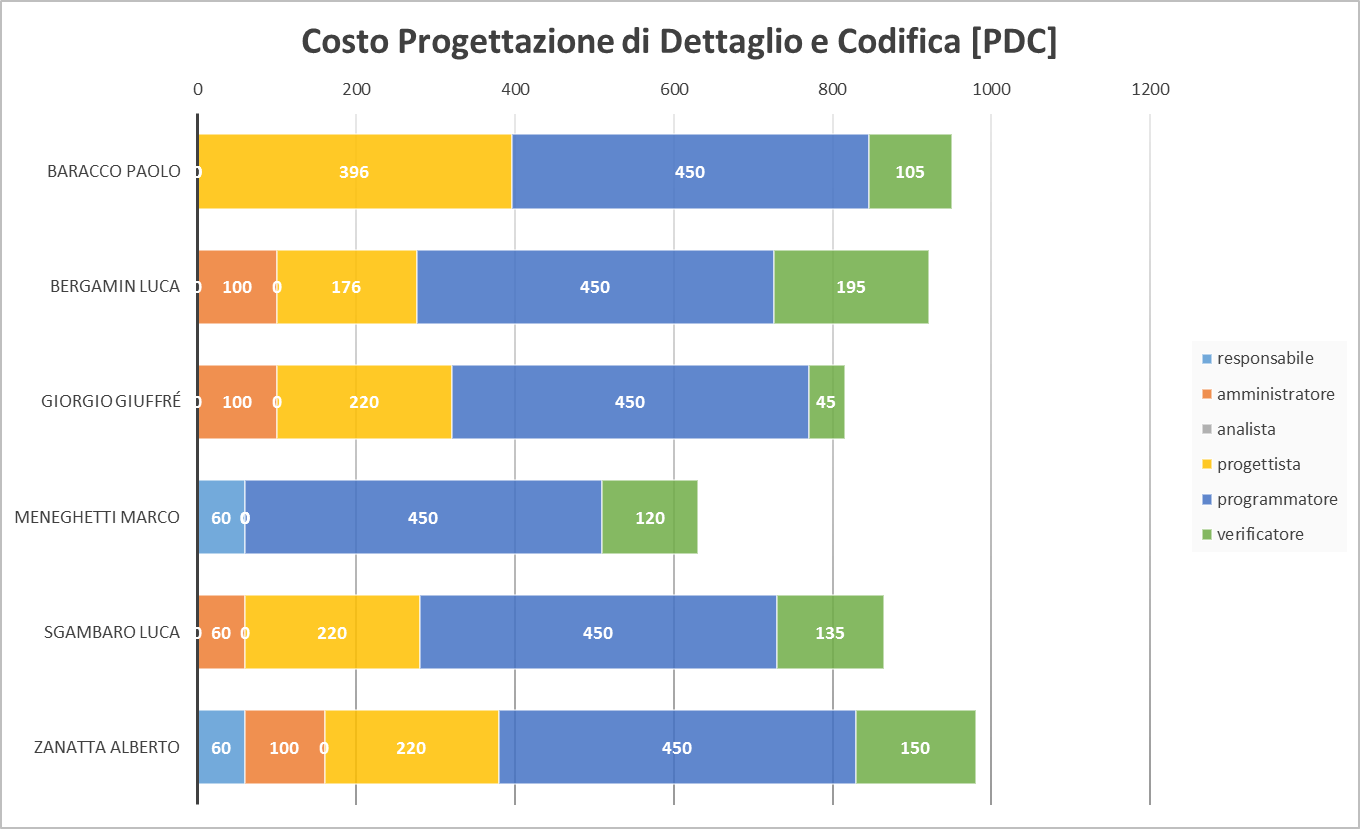
\includegraphics[width=1.2\textwidth]{img/costopdc.png}}
\label{tab:cpdc}

  \caption{Costo {\PDC} per ruolo, valori in euro (\euro).}
\end{figure}

\pagebreak[4]
\subsection{\VV}
\intropreventivo{\VV}

\begin{figure}[H]
\definecolor{white2}{rgb}{0.95,0.95,0.95}
\definecolor{white3}{rgb}{0.9,0.9,0.9}
%\rowcolors{1}{white}{white2}

\makebox[\textwidth][c]
{
  \begin{tabular}[width=1.2\textwidth]{ | l | c | c | c | c | c | c | r |}
    \hline
    \rowcolor[gray]{.9}
    Ruolo / persona & \R & \AM & \AN & \PJ & \PG & \V & Tot ore/persona \\ \hline
    \PB & 3 & 8 & 0 & 0 & 0 & 5 & 16 \\ \hline
    \LB & 3 & 0 & 0 & 0 & 0 & 2 & 5 \\ \hline
    \GG & 0 & 0 & 0 & 0 & 0 & 14 & 14 \\ \hline
    \MM & 0 & 0 & 2 & 0 & 0 & 15 & 17 \\ \hline
    \LS & 0 & 0 & 0 & 0 & 0 & 2 & 2 \\ \hline
    \AZ & 0 & 0 & 0 & 0 & 0 & 3 & 3 \\ \hline
    \rowcolor[gray]{.9}

    Totale ore/ruolo & 6 & 8 & 2 & 0 & 0 & 41 & 57 \\ \hline
    
  \end{tabular}
  }
  \caption{Ore/ruolo per persona nella fase di \VV.}
\label{fig:vv1}
\end{figure} 
% i colori danno problemi di visualizzazione alle linee

\pagebreak

\begin{figure}[H]
\makebox[\textwidth][c]{
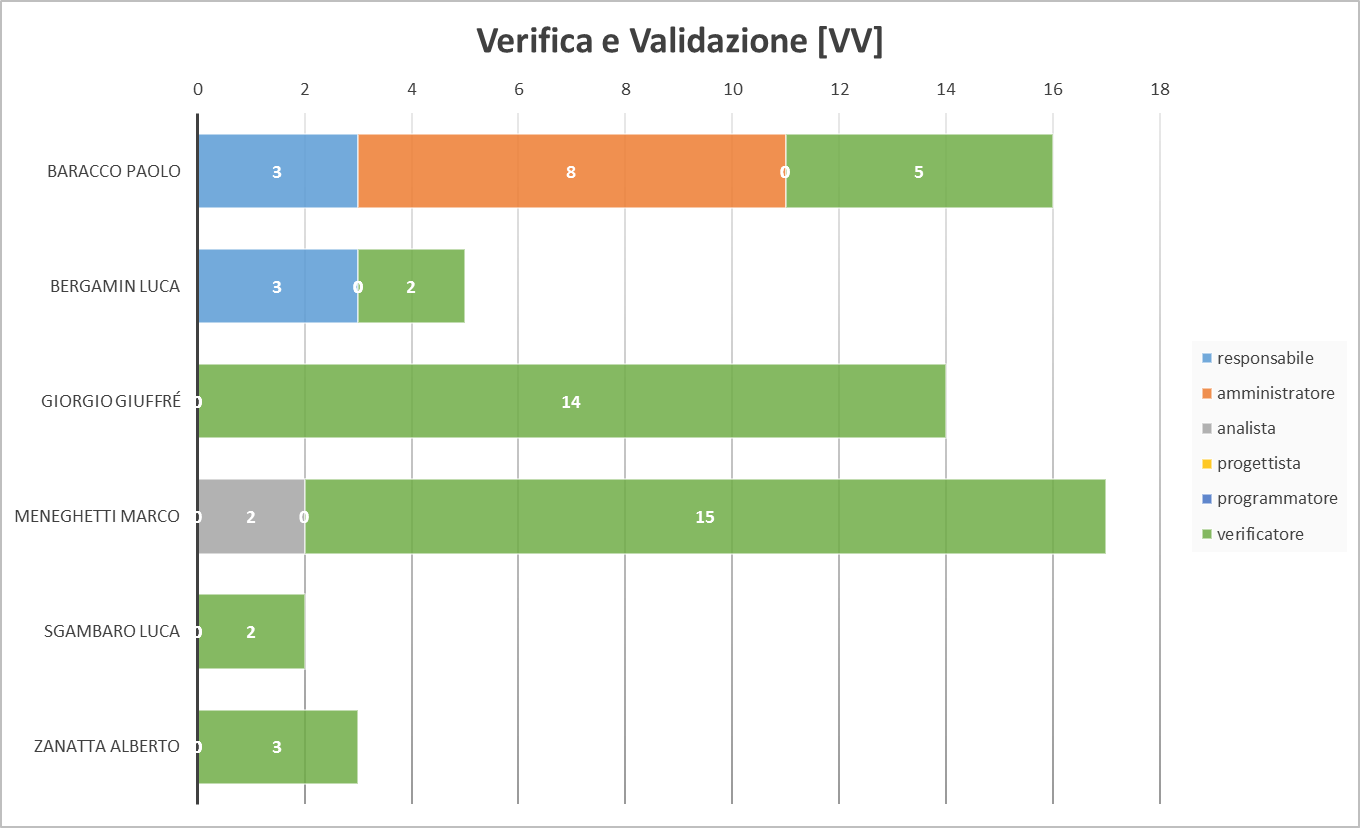
\includegraphics[width=1.1\textwidth]{img/orevv1.png}}
\caption{Ore/ruolo per persona nella fase di \VV.}
\label{fig:vv1}

\end{figure}

\begin{figure}[H]
\makebox[\textwidth][c]{
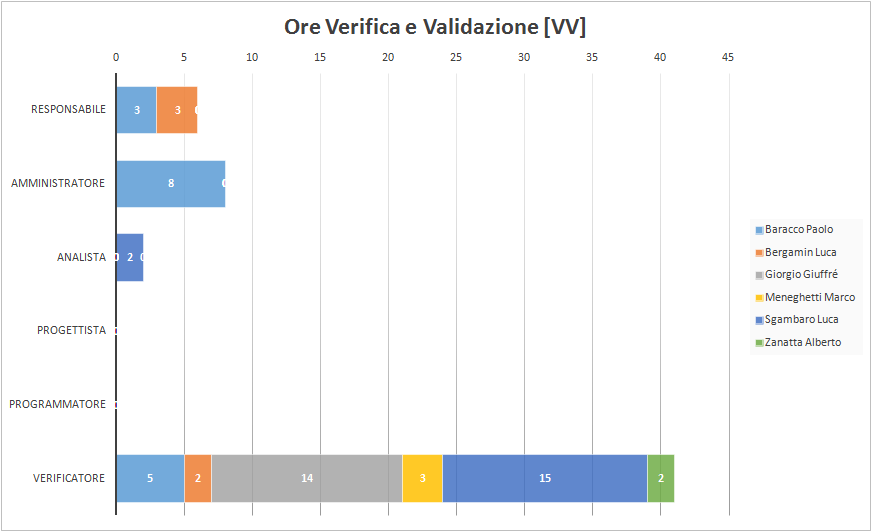
\includegraphics[width=1.1\textwidth]{img/orevv2.png}}
\caption{Ore/persona per ruolo nella fase di \VV.}
\label{fig:vv2}

\end{figure}


\pagebreak

\subsubsection{Costo \VV}
\introcosto{\VV}
Questa fase mira a completare tutte le attività di qualifica prefissate da {\hx}.

Gli sforzi maggiori si evidenziano nel ruolo di:
\begin{itemize}
\item {\Vx} per la verifica e validazione del prodotto creato.
\end{itemize}

\begin{figure}[H]
\makebox[\textwidth][c]
{
\definecolor{white2}{rgb}{0.95,0.95,0.95}
\definecolor{white3}{rgb}{0.9,0.9,0.9}
%\rowcolors{1}{white}{white2}

  \begin{tabular}{ | l | c | c | c | c | c | c | r |}
    \hline
    \rowcolor[gray]{.9}
    Ruolo / persona & \R & \AM & \AN & \PJ & \PG & \V & Tot euro/persona \\ \hline
    \PB & 90 & 160 & 0 & 0 & 0 & 75 & 325 \\ \hline
    \LB & 90 & 0 & 0 & 0 & 0 & 30 & 120 \\ \hline
    \GG & 0 & 0 & 0 & 0 & 0 & 210 & 210 \\ \hline
    \MM & 0 & 0 & 50 & 0 & 0 & 225 & 275 \\ \hline
    \LS & 0 & 0 & 0 & 0 & 0 & 30 & 30 \\ \hline
    \AZ & 0 & 0 & 0 & 0 & 0 & 45 & 45 \\ \hline
    \rowcolor[gray]{.9}

    Totale euro/ruolo & 180 & 160 & 50 & 0 & 0 & 615 & 1005 \\ \hline
  \end{tabular}
  
}\label{tab:vv}

  \caption{Tabella costo {\VV} per ruolo e per persona, valori in euro (\euro).}
\end{figure}

\begin{figure}[H]
\makebox[\textwidth][c]{
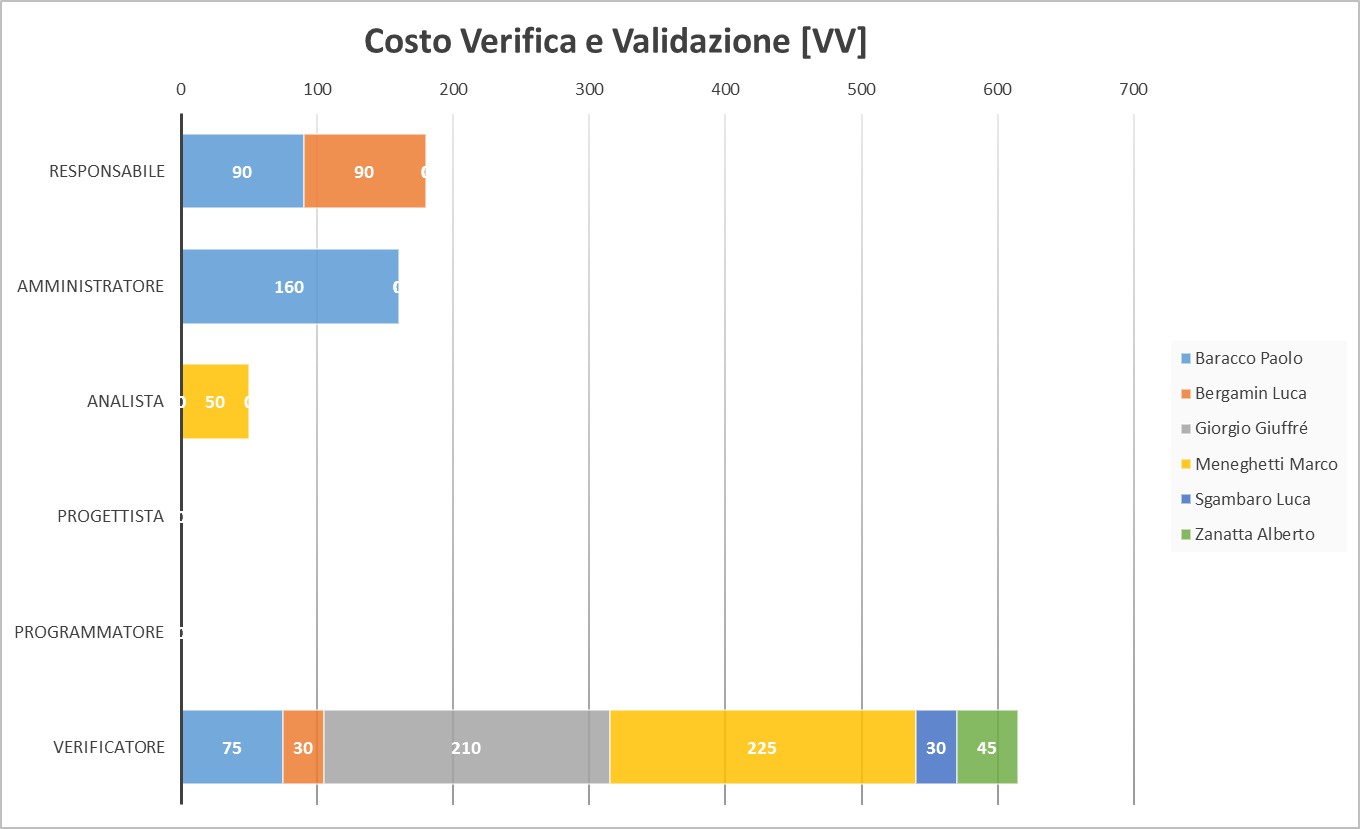
\includegraphics[width=1.2\textwidth]{img/costovv.png}}
\label{tab:cvv}

  \caption{Costo {\VV} per ruolo, valori in euro (\euro).}
\end{figure}

\pagebreak[4]

\subsection{Ore totali del progetto}
Di seguito si riporta la divisione oraria pianificata generale.

Successivamente sono evidenziate graficamente la divisione delle ore per persona e ruolo.

Questo quadro riassuntivo include il periodo di {\AR}, il quale \textbf{non è a carico del cliente}.

{\hx} complessivamente ritiene di aver diviso equamente il carico di lavoro. Ogni disparità a livello di periodo è bilanciata nei periodi successivi. 

Il quantitativo preventivato a persona è fissato in \textbf{138 ore} e il quantitativo di ore preventivate totali è fissato a \textbf{828 ore}.

Si è raggiunto l'obiettivo prefissato di assegnare ogni ruolo a ciascun componente di {\hx} almeno una volta. Disparità in questo senso sono inevitabili: inevitabilmente è necessaria una o più "figure di riferimento" per ogni ruolo, che impieghino più risorse per raggiungere gli incarichi più gravosi.


\begin{figure}[H]
\definecolor{white2}{rgb}{0.95,0.95,0.95}
\definecolor{white3}{rgb}{0.9,0.9,0.9}
%\rowcolors{1}{white}{white2}

\makebox[\textwidth][c]
{
  \begin{tabular}[width=1.2\textwidth]{ | l | c | c | c | c | c | c | r |}
    \hline
    \rowcolor[gray]{.9}
    Ruolo / persona & \R & \AM & \AN & \PJ & \PG & \V & Tot ore/persona \\ \hline
    \PB & 10 & 11 & 14 & 48 & 30 & 25 & 138 \\ \hline
    \LB & 15 & 19 & 6 & 46 & 30 & 22 & 138 \\ \hline
    \GG & 3 & 29 & 8 & 45 & 30 & 23 & 138 \\ \hline
    \MM & 2 & 20 & 10 & 45 & 30 & 31 & 138 \\ \hline
    \LS & 2 & 5 & 17 & 50 & 30 & 34 & 138 \\ \hline
    \AZ & 3 & 9 & 21 & 46 & 30 & 29 & 138 \\ \hline
    \rowcolor[gray]{.9}

    Totale ore/ruolo & 35 & 93 & 76 & 280 & 180 & 164 & 828 \\ \hline
    
  \end{tabular}
  }
  
  \label{tab:gen}

  \caption{Tabella costo generale per ruolo e per persona, valori in euro (\euro).}
\end{figure} 
% i colori danno problemi di visualizzazione alle linee


È possibile ricavare interessanti statistiche dalla tabella (\ref{tab:gen}) e dal grafico di ripartizione oraria (\ref{fig:gen2}): % che riferimento ha inserito latex?
\begin{itemize}
\item Il ruolo {\Rx} richiede il quantitativo di ore minimo rispetto alle altre mansioni: inizialmente è richiesto uno sforzo maggiore per la stesura del \emph{Piano di Progetto}, ma superata la fase di {\AR} questo ruolo è richiesto in misura minore.
\item Il ruolo {\AMx} richiede una discreta quantità di ore soprattutto in fase di {\AR} per definire un ambiente di sviluppo ideale. Completata questa fase il ruolo è richiesto in misura minore.
\item Il ruolo {\ANx} richiede anch'esso la maggior parte delle ore in fase di {\AR} e successivamente sono ammessi solo incrementi del documento di {\AR}.
\item Il ruolo {\PJx} è ritenuto da {\hx} cruciale, dunque ne è stato assegnato il quantitativo maggiore di ore.
\item Il ruolo {\PGx} richiede una quantità di tempo pari a circa due terzi delle ore impiegate in fase di progettazione. Questa divisione a livello di preventivo è stata ritenuta accettabile, ma {\hx} si riserva di effettuare nuovamente questa analisi alla consegna del consuntivo finale.
\item Il ruolo {\Vx} richiede una quantità di tempo simile a quella riservata per il ruolo di {\PGx} e questa assegnazione è sembrata accettabile a livello di preventivo. {\hx} si riserva di effettuare nuovamente questa analisi alla consegna del consuntivo finale.
\end{itemize}



\pagebreak

\begin{figure}[H]
\makebox[\textwidth][c]{
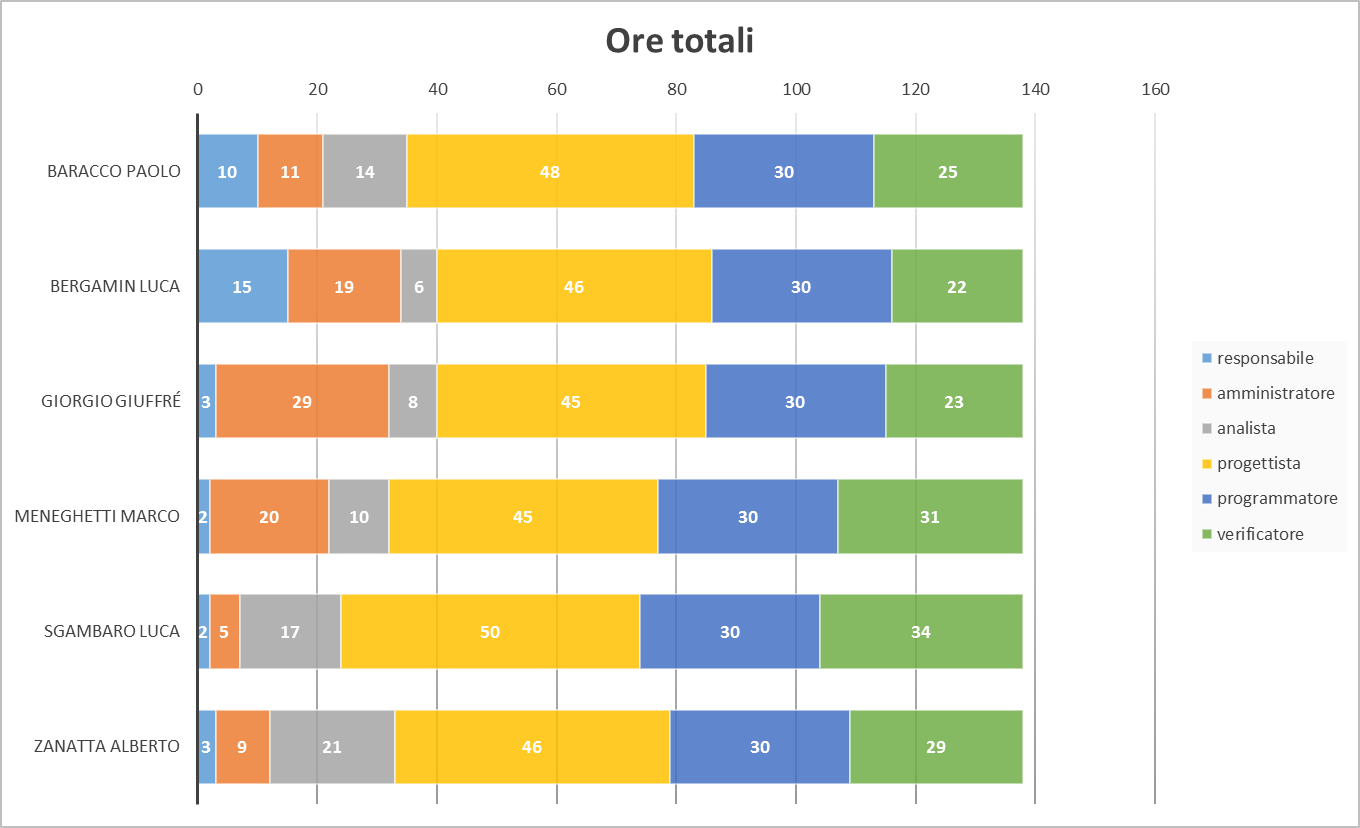
\includegraphics[width=1.1\textwidth]{img/oretotali1.png}}
\caption{Ore/ruolo per persona per il progetto {\proj}.}
\label{fig:gen1}

\end{figure}

\begin{figure}[H]
\makebox[\textwidth][c]{
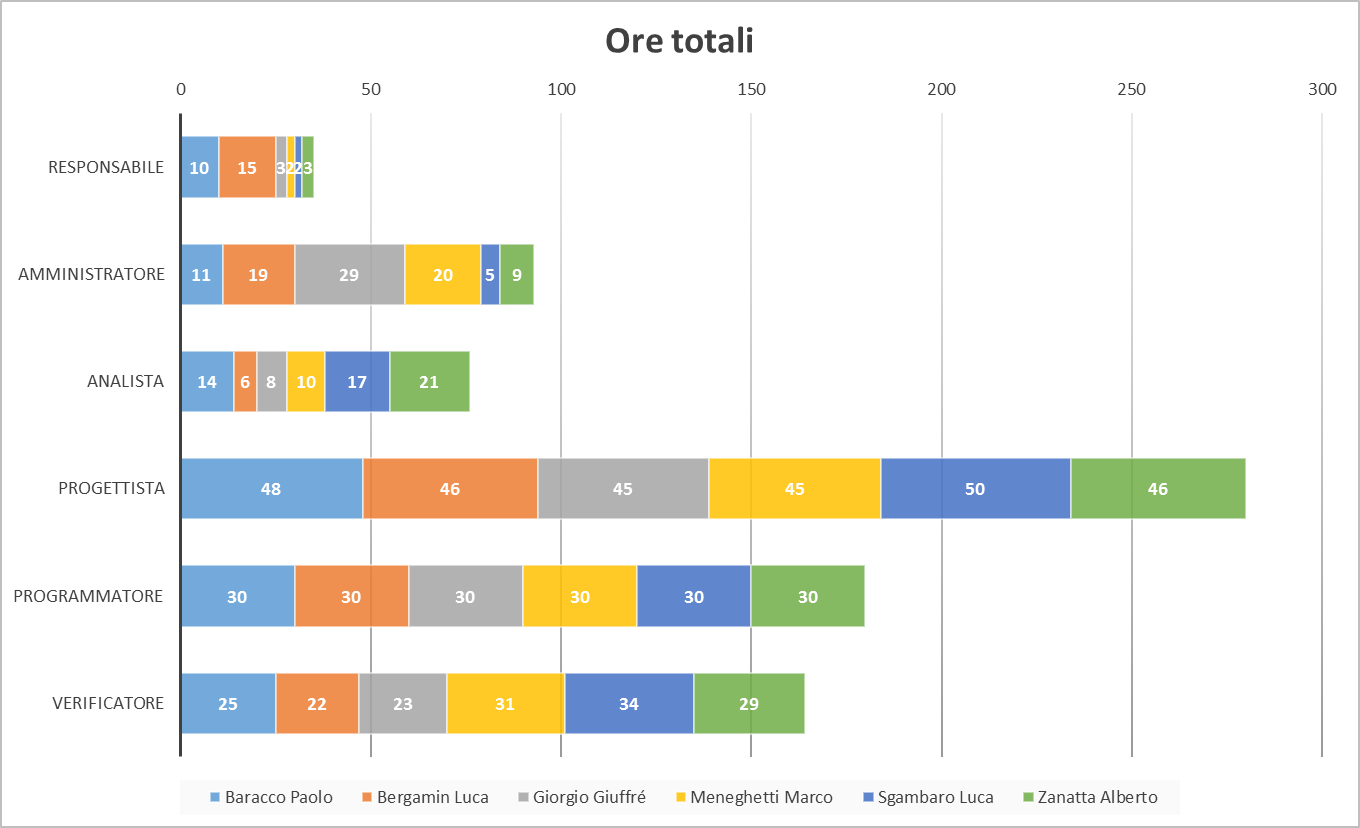
\includegraphics[width=1.1\textwidth]{img/oretotali2.png}}
\caption{Ore/persona per ruolo per il progetto {\proj}.}
\label{fig:gen2}

\end{figure}


\subsubsection{Costo ore totali del progetto}
Di seguito si riporta il costo delle ore totali, suddiviso per persona e ruolo.

Questo quadro riassuntivo include il periodo di {\AR}, il quale \textbf{non è a carico del cliente}.

\begin{figure}[H]
\makebox[\textwidth][c]
{
\definecolor{white2}{rgb}{0.95,0.95,0.95}
\definecolor{white3}{rgb}{0.9,0.9,0.9}
%\rowcolors{1}{white}{white2}

  \begin{tabular}{ | l | c | c | c | c | c | c | r |}
    \hline
    \rowcolor[gray]{.9}
    Ruolo / persona & \R & \AM & \AN & \PJ & \PG & \V & Tot euro/persona \\ \hline
    \PB & 330 & 220 & 350 & 1056 & 450 & 375 & 2751 \\ \hline
    \LB & 450 & 380 & 150 & 1012 & 450 & 330 & 2772 \\ \hline
    \GG & 90 & 580 & 200 & 990 & 450 & 345 & 2655 \\ \hline
    \MM & 60 & 400 & 250 & 990 & 450 & 465 & 2615 \\ \hline
    \LS & 60 & 100 & 425 & 1100 & 450 & 510 & 2645 \\ \hline
    \AZ & 90 & 180 & 525 & 1012 & 450 & 435 & 2692 \\ \hline
    \rowcolor[gray]{.9}

    Totale euro/ruolo & 1050 & 1860 & 1900 & 6160 & 2700 & 2460 & 16130 \\ \hline
  \end{tabular}
  
}\label{tab:cgen}

  \caption{Tabella costo totale per ruolo e per persona, valori in euro (\euro).}
\end{figure}

\begin{figure}[H]
\makebox[\textwidth][c]{
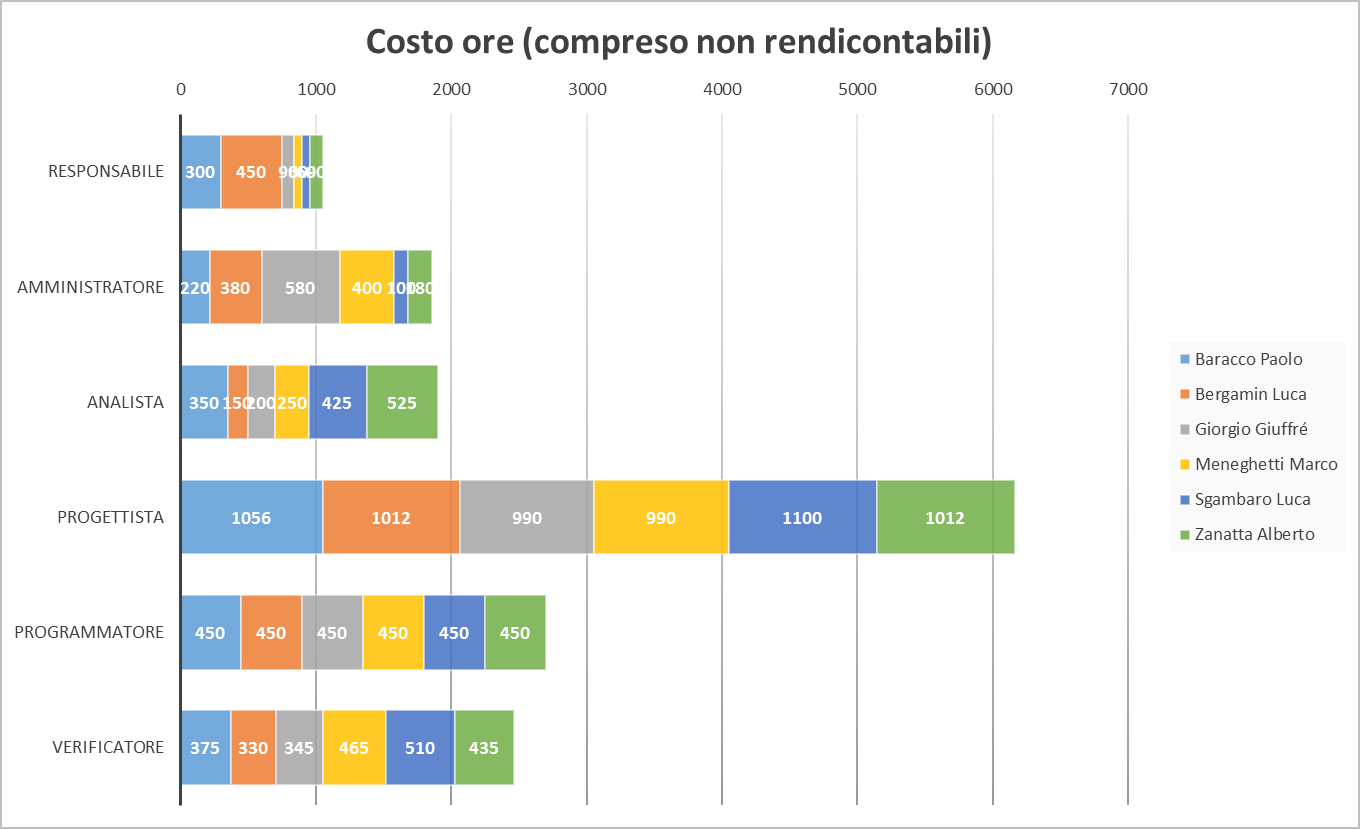
\includegraphics[width=1.2\textwidth]{img/costototale.png}}
\label{tab:cgen1}

  \caption{Costo totale per il progetto {\proj} per ruolo e per persona, valori in euro (\euro).}
\end{figure}


%si riporta pure oretotali4.png?
\pagebreak[4]



\subsection{Ore rendicontate del progetto} 
\label{sec:orerend}
%stessa cosa della sezione precedente
Di seguito si riporta la divisione oraria pianificata generale delle sole ore rendicontate.

Successivamente sono evidenziate graficamente la divisione delle ore per persona e ruolo.

Questo quadro riassuntivo esclude il periodo di {\AR}: il totale risultante \textbf{è a carico del cliente}.

Il quantitativo rendicontato a preventivo a persona varia tra le \textbf{103} e \textbf{108 ore} e il quantitativo di ore preventivate totali è fissato a \textbf{634 ore}.

{\hx} complessivamente ritiene di aver diviso equamente il carico di lavoro, in quanto i scostamenti orari in misura minore del 5\%.

\begin{figure}[H]
\definecolor{white2}{rgb}{0.95,0.95,0.95}
\definecolor{white3}{rgb}{0.9,0.9,0.9}
%\rowcolors{1}{white}{white2}

\makebox[\textwidth][c]
{
  \begin{tabular}[width=1.2\textwidth]{ | l | c | c | c | c | c | c | r |}
    \hline
    \rowcolor[gray]{.9}
    Ruolo / persona & \R & \AM & \AN & \PJ & \PG & \V & Tot ore/persona \\ \hline
    \PB & 3 & 8 & 0 & 48 & 30 & 18 & 107 \\ \hline
    \LB & 3 & 8 & 0 & 46 & 30 & 16 & 103 \\ \hline
    \GG & 3 & 5 & 0 & 45 & 30 & 20 & 103 \\ \hline
    \MM & 2 & 0 & 2 & 45 & 30 & 27 & 106 \\ \hline
    \LS & 2 & 3 & 5 & 50 & 30 & 17 & 107 \\ \hline
    \AZ & 2 & 5 & 8 & 46 & 30 & 17 & 108 \\ \hline
    \rowcolor[gray]{.9}

    Totale ore/ruolo & 35 & 93 & 76 & 280 & 180 & 164 & 828 \\ \hline
    
  \end{tabular}
  }
  
  \label{tab:rend}

  \caption{Tabella costo generale per ruolo e per persona, valori in euro (\euro).}
\end{figure} 
% i colori danno problemi di visualizzazione alle linee


\subsubsection{Costo ore rendicontate del progetto}
Di seguito si riporta il costo delle ore totali rendicontate, suddiviso per persona e ruolo.

Questo quadro riassuntivo esclude il periodo di {\AR}: i costi che seguono \textbf{ sono a carico del cliente}.

\begin{figure}[H]
\makebox[\textwidth][c]
{
\definecolor{white2}{rgb}{0.95,0.95,0.95}
\definecolor{white3}{rgb}{0.9,0.9,0.9}
%\rowcolors{1}{white}{white2}

  \begin{tabular}{ | l | c | c | c | c | c | c | r |}
    \hline
    \rowcolor[gray]{.9}
    Ruolo / persona & \R & \AM & \AN & \PJ & \PG & \V & Tot euro/persona \\ \hline
    \PB & 90 & 160 & 0 & 1056 & 450 & 270 & 2026 \\ \hline
    \LB & 90 & 160 & 0 & 1012 & 450 & 240 & 1952 \\ \hline
    \GG & 90 & 100 & 0 & 990 & 450 & 300 & 1930 \\ \hline
    \MM & 60 & 0 & 50 & 990 & 450 & 405 & 1955 \\ \hline
    \LS & 60 & 60 & 125 & 1100 & 450 & 255 & 2050 \\ \hline
    \AZ & 60 & 100 & 200 & 1012 & 450 & 255 & 2077 \\ \hline
    \rowcolor[gray]{.9}

    Totale euro/ruolo & 450 & 580 & 375 & 6160 & 2700 & 1725 & 11990 \\ \hline
  \end{tabular}
  
}\label{tab:cgen}

  \caption{Tabella costo totale per ruolo e per persona, valori in euro (\euro).}
\end{figure}

Il costo totale del progetto {\proj} preventivato è arrotondato a \textbf{12000{\euro}} (\emph{dodicimila euro}).

\begin{figure}[H]
\makebox[\textwidth][c]{
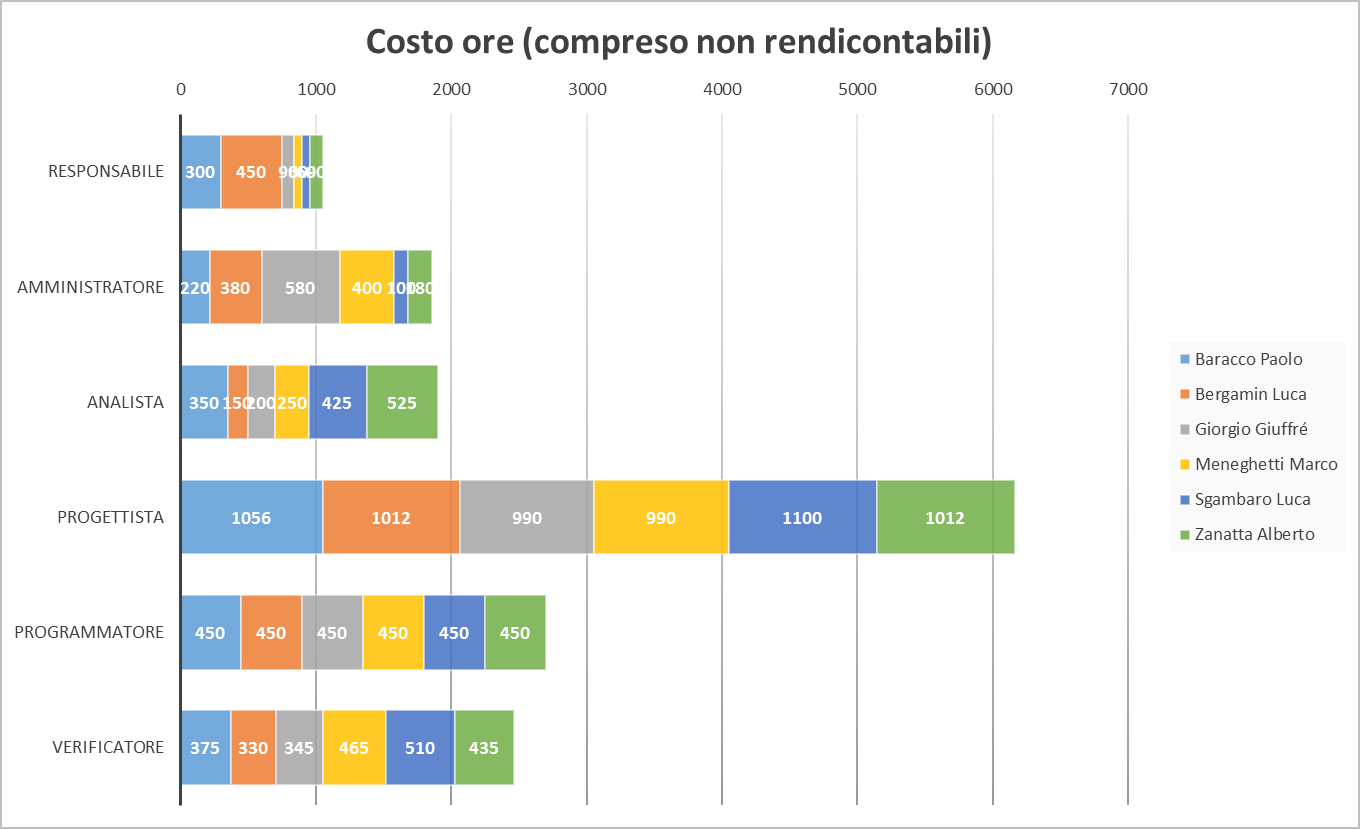
\includegraphics[width=1.2\textwidth]{img/costototale.png}}
\label{tab:cgen1}

  \caption{Costo totale per il progetto {\proj} per ruolo e per persona, valori in euro (\euro).}
\end{figure}

\pagebreak
\section{Consuntivo di periodo} \label{sec:consuntivo}
In questa sezione sono indicate le spese affrontate a termine di ogni \gloss{milestone} interna. Queste andranno a sommarsi per infine stilare il consuntivo finale.



\newcommand{\introconsuntivo}[1]
{
Di seguito si riporta la divisione oraria effettivamente adottata nella fase di #1.

Successivamente sono evidenziate graficamente la divisione delle ore per persona e per ruolo. 

È inoltre riportata la variazione riportata rispetto alla \gloss{baseline} inizialmente stilata e infine l'eventuale variazione di costo rispetto al preventivo.
}

\subsection{Consuntivo \AR}
\introconsuntivo{\AR}

Si ricorda che questo costo viene fornito a scopo informativo e rappresenta l'investimento effettuato da {\hx} prima dell'aggiudicazione dell'appalto e perciò tale periodo \textbf{non è a carico del cliente}. 

\subsubsection{Variazioni nella pianificazione}

\begin{figure}[H]
\makebox[\textwidth][c]{
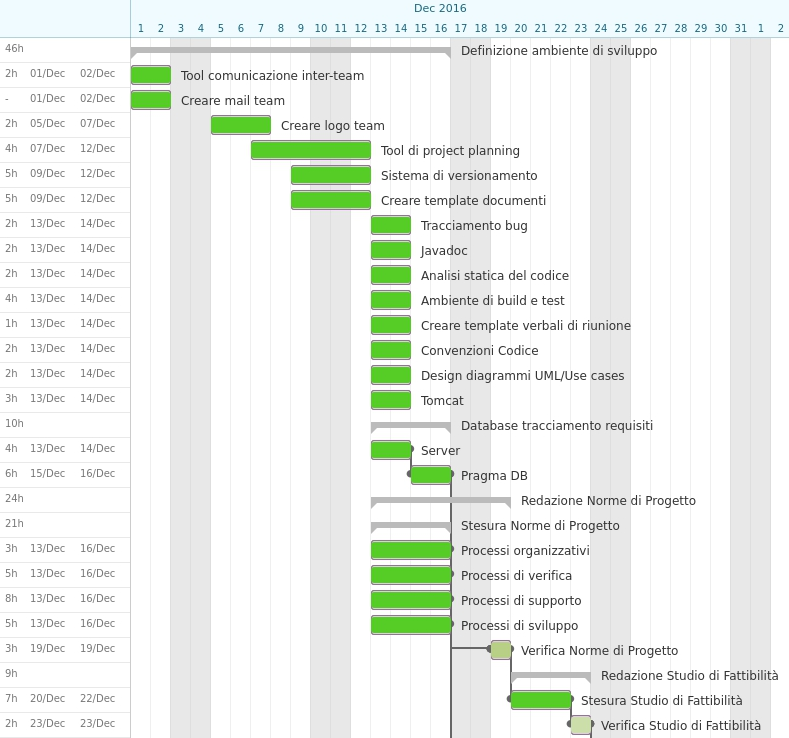
\includegraphics[width=1.2\textwidth]{img/ganttarc1.png}}
\label{tab:cgen1}

  \caption{Variazione rispetto alla pianificazione per fase di \AR, diagramma di Gantt (parte 1)}
\end{figure}


\begin{figure}[H]
\makebox[\textwidth][c]{
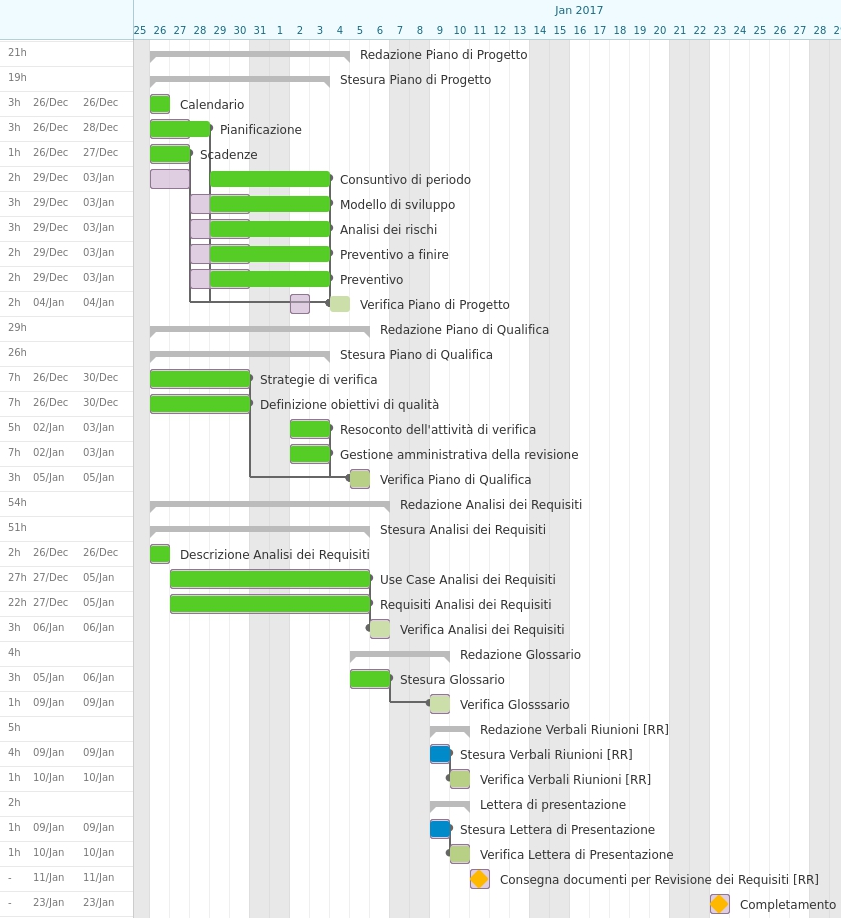
\includegraphics[width=1.2\textwidth]{img/ganttarc2.png}}
\label{tab:cgen1}

  \caption{Variazione rispetto alla pianificazione per fase di \AR, diagramma di Gantt (parte 2)}
\end{figure}

Si è verificato un ritardo nella stesura del presente documento a causa di una influenza di un membro del gruppo in data 30-12-2016.

Questo ha portato un ritardo complessivo pari a 3 giorni rispetto alla \gloss{baseline}; tuttavia il task, non presentando dipendenze, non ha portato ritardi se non all'attività di verifica relativa al documento stesso.

\subsubsection{Variazione nei costi}
\begin{itemize}

\item Non sono state rilevate variazioni nei costi.

\item Non si riportano i grafici di variazione oraria.

\item Si riportano le tabelle di divisione oraria effettive e i relativi costi.

\end{itemize}
% i colori danno problemi di visualizzazione alle linee
\begin{figure}[H]
\makebox[\textwidth][c]
{
\definecolor{white2}{rgb}{0.95,0.95,0.95}
\definecolor{white3}{rgb}{0.9,0.9,0.9}
%\rowcolors{1}{white}{white2}

  \begin{tabular}{ | l | c | c | c | c | c | c | r |}
    \hline
    \rowcolor[gray]{.9}
    Ruolo / persona & \R & \AM & \AN & \PJ & \PG & \V & Tot ore/persona \\ \hline
    \PB & 7 & 3 & 14 & 0 & 0 & 7 & 31 \\ \hline
    \LB & 12 & 11 & 6 & 0 & 0 & 6 & 35 \\ \hline
    \GG & 0 & 24 & 8 & 0 & 0 & 3 & 35 \\ \hline
    \MM & 0 & 20 & 8 & 0 & 0 & 4 & 32\\ \hline
    \LS & 0 & 2 & 12 & 0 & 0 & 17 & 31\\ \hline
    \AZ & 1 & 4 & 13 & 0 & 0 & 12 & 30 \\ \hline
    \rowcolor[gray]{.9}

    Totale ore/ruolo & 20 & 64 & 61 & 0 & 0 & 49 & 194 \\ \hline
    
  \end{tabular}
}
\label{tab:car}
\caption{Tabella ore effettive {\AR} per ruolo e per persona.}

\end{figure}


\begin{figure}[H]
\makebox[\textwidth][c]
{
\definecolor{white2}{rgb}{0.95,0.95,0.95}
\definecolor{white3}{rgb}{0.9,0.9,0.9}
%\rowcolors{1}{white}{white2}

  \begin{tabular}{ | l | c | c | c | c | c | c | r |}
    \hline
    \rowcolor[gray]{.9}
    Ruolo / persona & \R & \AM & \AN & \PJ & \PG & \V & Tot euro/persona \\ \hline
    \PB & 210 & 60 & 350 & 0 & 0 & 105 & 725 \\ \hline
    \LB & 360 & 220 & 150 & 0 & 0 & 90 & 820 \\ \hline
    \GG & 0 & 480 & 200 & 0 & 0 & 45 & 725 \\ \hline
    \MM & 0 & 400 & 200 & 0 & 0 & 60 & 660 \\ \hline
    \LS & 0 & 40 & 300 & 0 & 0 & 255 & 595 \\ \hline
    \AZ & 30 & 80 & 325 & 0 & 0 & 180 & 615 \\ \hline
    \rowcolor[gray]{.9}

    Totale euro/ruolo & 600 & 1280 & 1525 & 0 & 0 & 735 & 4140 \\ \hline
  \end{tabular}
  
}
\label{tab:car}
\caption{Tabella costo effettivo {\AR} per ruolo e per persona, valori in euro (\euro).}
\end{figure}

\subsubsection{Preventivo a finire}
Siccome non sono state rilevate variazioni nei costi, il preventivo a finire (a carico del cliente) è pari a quelle riportate nella sezione \ref{sec:orerend} \nameref{sec:orerend}.

\pagebreak
\section{Organigramma}	\label{sec:organigramma}
\subsection{Redazione}

\begin{figure}[H]
\makebox[\textwidth][c]
{
  \begin{tabular}{ | c | c | c |}
			\hline
			\textbf{Nominativo} & \textbf{Data di redazione} & \textbf{Firma} \\
			\hline
			\LB & 25-12-2016 &   \myincludegraphics{img/firmalb.jpg}\\
			\hline
  \end{tabular}
}
\caption{Redazione}
\end{figure}

\subsection{Approvazione}
\begin{figure}[H]
\makebox[\textwidth][c]
{
  \begin{tabular}{ | c | c | c |}
			\hline
			\textbf{Nominativo}     & \textbf{Data di approvazione} & \textbf{Firma}  \\
			\hline
			\LB		& 24-01-2017	&  \myincludegraphics{img/firmalb.jpg}	\\
			\hline
			\TV	          &		           &			\\
			\hline
\end{tabular}
}
\caption{Approvazione}
\end{figure}

\subsection{Accettazione dei componenti}
\begin{figure}[H]
\makebox[\textwidth][c]
{
  \begin{tabular}{ | c | c | c |}
			\hline
			\textbf{Nominativo} & \textbf{Data} & \textbf{Firma} \\
			\hline
			\AZ		&	24-01-2017	&  \myincludegraphics{img/firmaaz.jpg}	\\
			\hline
			\GG		&	24-01-2017   &  \myincludegraphics[scale=0.75]{img/firmagg.png}	\\
			\hline
			\LB		&	24-01-2017	&  \myincludegraphics{img/firmalb.jpg}		\\
			\hline
			\LS		&	24-01-2017	&  \myincludegraphics{img/firmals.jpg}		\\
			\hline
			\MM		&	24-01-2017	&  \myincludegraphics{img/firmamm.png}		\\
			\hline
			\PB		&	24-01-2017	&  \myincludegraphics{img/firmapb.png}		\\
			\hline
\end{tabular}
}
\caption{Accettazione}
\end{figure}

\subsection{Componenti}
\begin{figure}[H]
\makebox[\textwidth][c]
{
  \begin{tabular}{ | c | c | c | c |}
			\hline
			\textbf{Nominativo} & \textbf{Matricola} & \raggedright \textbf{Indirizzo di posta elettronica} & \textbf{Ruoli} \\[1ex]
			\hline
	 		\AZ	& 1100543	& \href{mailto:alberto.zanatta.3@studenti.unipd.it}{alberto.zanatta.3@studenti.unipd.it} 	& \AN,  \V	\\[1ex]
			\hline
			\GG		& 1069456	& \href{mailto:giorgio.giuffre@studenti.unipd.it}{giorgio.giuffre@studenti.unipd.it} 	&  \AN, \AM, \V	\\[1ex]
			\hline
			\LB		& 1097055	& \href{mailto:luca.bergamin.3@studenti.unipd.it}{luca.bergamin.3@studenti.unipd.it}  &  \AN, \R, \V \\[1ex]
			\hline
			\LS 		& 1099154	& \href{mailto:luca.sgambaro@studenti.unipd.it}{luca.sgambaro@studenti.unipd.it} 	& \AN, \V	\\[1ex]
			\hline
			\MM		& 1097051	& \href{mailto:marco.meneghetti.5@studenti.unipd.it}{marco.meneghetti.5@studenti.unipd.it} & \AN, \AM, \V	\\[1ex]
			\hline
			\PB		& 1097928	& \href{mailto:paolo.baracco.1@studenti.unipd.it}{paolo.baracco.1@studenti.unipd.it} 	&  \AN, \R, \V 	\\[1ex]
			\hline
\end{tabular}
}
\caption{Componenti}
\end{figure}

\end{document}
